% Generated by Sphinx.
\def\sphinxdocclass{report}
\documentclass[letterpaper,10pt,english]{sphinxmanual}
\usepackage[utf8]{inputenc}
\DeclareUnicodeCharacter{00A0}{\nobreakspace}
\usepackage{cmap}
\usepackage[T1]{fontenc}
\usepackage{babel}
\usepackage{times}
\usepackage[Bjarne]{fncychap}
\usepackage{longtable}
\usepackage{sphinx}
\usepackage{multirow}


\title{OpenMOOC Guide: Creating Courses}
\date{September 08, 2014}
\release{}
\author{}
\newcommand{\sphinxlogo}{}
\renewcommand{\releasename}{Release}
\makeindex

\makeatletter
\def\PYG@reset{\let\PYG@it=\relax \let\PYG@bf=\relax%
    \let\PYG@ul=\relax \let\PYG@tc=\relax%
    \let\PYG@bc=\relax \let\PYG@ff=\relax}
\def\PYG@tok#1{\csname PYG@tok@#1\endcsname}
\def\PYG@toks#1+{\ifx\relax#1\empty\else%
    \PYG@tok{#1}\expandafter\PYG@toks\fi}
\def\PYG@do#1{\PYG@bc{\PYG@tc{\PYG@ul{%
    \PYG@it{\PYG@bf{\PYG@ff{#1}}}}}}}
\def\PYG#1#2{\PYG@reset\PYG@toks#1+\relax+\PYG@do{#2}}

\expandafter\def\csname PYG@tok@gd\endcsname{\def\PYG@tc##1{\textcolor[rgb]{0.63,0.00,0.00}{##1}}}
\expandafter\def\csname PYG@tok@gu\endcsname{\let\PYG@bf=\textbf\def\PYG@tc##1{\textcolor[rgb]{0.50,0.00,0.50}{##1}}}
\expandafter\def\csname PYG@tok@gt\endcsname{\def\PYG@tc##1{\textcolor[rgb]{0.00,0.27,0.87}{##1}}}
\expandafter\def\csname PYG@tok@gs\endcsname{\let\PYG@bf=\textbf}
\expandafter\def\csname PYG@tok@gr\endcsname{\def\PYG@tc##1{\textcolor[rgb]{1.00,0.00,0.00}{##1}}}
\expandafter\def\csname PYG@tok@cm\endcsname{\let\PYG@it=\textit\def\PYG@tc##1{\textcolor[rgb]{0.25,0.50,0.56}{##1}}}
\expandafter\def\csname PYG@tok@vg\endcsname{\def\PYG@tc##1{\textcolor[rgb]{0.73,0.38,0.84}{##1}}}
\expandafter\def\csname PYG@tok@m\endcsname{\def\PYG@tc##1{\textcolor[rgb]{0.13,0.50,0.31}{##1}}}
\expandafter\def\csname PYG@tok@mh\endcsname{\def\PYG@tc##1{\textcolor[rgb]{0.13,0.50,0.31}{##1}}}
\expandafter\def\csname PYG@tok@cs\endcsname{\def\PYG@tc##1{\textcolor[rgb]{0.25,0.50,0.56}{##1}}\def\PYG@bc##1{\setlength{\fboxsep}{0pt}\colorbox[rgb]{1.00,0.94,0.94}{\strut ##1}}}
\expandafter\def\csname PYG@tok@ge\endcsname{\let\PYG@it=\textit}
\expandafter\def\csname PYG@tok@vc\endcsname{\def\PYG@tc##1{\textcolor[rgb]{0.73,0.38,0.84}{##1}}}
\expandafter\def\csname PYG@tok@il\endcsname{\def\PYG@tc##1{\textcolor[rgb]{0.13,0.50,0.31}{##1}}}
\expandafter\def\csname PYG@tok@go\endcsname{\def\PYG@tc##1{\textcolor[rgb]{0.20,0.20,0.20}{##1}}}
\expandafter\def\csname PYG@tok@cp\endcsname{\def\PYG@tc##1{\textcolor[rgb]{0.00,0.44,0.13}{##1}}}
\expandafter\def\csname PYG@tok@gi\endcsname{\def\PYG@tc##1{\textcolor[rgb]{0.00,0.63,0.00}{##1}}}
\expandafter\def\csname PYG@tok@gh\endcsname{\let\PYG@bf=\textbf\def\PYG@tc##1{\textcolor[rgb]{0.00,0.00,0.50}{##1}}}
\expandafter\def\csname PYG@tok@ni\endcsname{\let\PYG@bf=\textbf\def\PYG@tc##1{\textcolor[rgb]{0.84,0.33,0.22}{##1}}}
\expandafter\def\csname PYG@tok@nl\endcsname{\let\PYG@bf=\textbf\def\PYG@tc##1{\textcolor[rgb]{0.00,0.13,0.44}{##1}}}
\expandafter\def\csname PYG@tok@nn\endcsname{\let\PYG@bf=\textbf\def\PYG@tc##1{\textcolor[rgb]{0.05,0.52,0.71}{##1}}}
\expandafter\def\csname PYG@tok@no\endcsname{\def\PYG@tc##1{\textcolor[rgb]{0.38,0.68,0.84}{##1}}}
\expandafter\def\csname PYG@tok@na\endcsname{\def\PYG@tc##1{\textcolor[rgb]{0.25,0.44,0.63}{##1}}}
\expandafter\def\csname PYG@tok@nb\endcsname{\def\PYG@tc##1{\textcolor[rgb]{0.00,0.44,0.13}{##1}}}
\expandafter\def\csname PYG@tok@nc\endcsname{\let\PYG@bf=\textbf\def\PYG@tc##1{\textcolor[rgb]{0.05,0.52,0.71}{##1}}}
\expandafter\def\csname PYG@tok@nd\endcsname{\let\PYG@bf=\textbf\def\PYG@tc##1{\textcolor[rgb]{0.33,0.33,0.33}{##1}}}
\expandafter\def\csname PYG@tok@ne\endcsname{\def\PYG@tc##1{\textcolor[rgb]{0.00,0.44,0.13}{##1}}}
\expandafter\def\csname PYG@tok@nf\endcsname{\def\PYG@tc##1{\textcolor[rgb]{0.02,0.16,0.49}{##1}}}
\expandafter\def\csname PYG@tok@si\endcsname{\let\PYG@it=\textit\def\PYG@tc##1{\textcolor[rgb]{0.44,0.63,0.82}{##1}}}
\expandafter\def\csname PYG@tok@s2\endcsname{\def\PYG@tc##1{\textcolor[rgb]{0.25,0.44,0.63}{##1}}}
\expandafter\def\csname PYG@tok@vi\endcsname{\def\PYG@tc##1{\textcolor[rgb]{0.73,0.38,0.84}{##1}}}
\expandafter\def\csname PYG@tok@nt\endcsname{\let\PYG@bf=\textbf\def\PYG@tc##1{\textcolor[rgb]{0.02,0.16,0.45}{##1}}}
\expandafter\def\csname PYG@tok@nv\endcsname{\def\PYG@tc##1{\textcolor[rgb]{0.73,0.38,0.84}{##1}}}
\expandafter\def\csname PYG@tok@s1\endcsname{\def\PYG@tc##1{\textcolor[rgb]{0.25,0.44,0.63}{##1}}}
\expandafter\def\csname PYG@tok@gp\endcsname{\let\PYG@bf=\textbf\def\PYG@tc##1{\textcolor[rgb]{0.78,0.36,0.04}{##1}}}
\expandafter\def\csname PYG@tok@sh\endcsname{\def\PYG@tc##1{\textcolor[rgb]{0.25,0.44,0.63}{##1}}}
\expandafter\def\csname PYG@tok@ow\endcsname{\let\PYG@bf=\textbf\def\PYG@tc##1{\textcolor[rgb]{0.00,0.44,0.13}{##1}}}
\expandafter\def\csname PYG@tok@sx\endcsname{\def\PYG@tc##1{\textcolor[rgb]{0.78,0.36,0.04}{##1}}}
\expandafter\def\csname PYG@tok@bp\endcsname{\def\PYG@tc##1{\textcolor[rgb]{0.00,0.44,0.13}{##1}}}
\expandafter\def\csname PYG@tok@c1\endcsname{\let\PYG@it=\textit\def\PYG@tc##1{\textcolor[rgb]{0.25,0.50,0.56}{##1}}}
\expandafter\def\csname PYG@tok@kc\endcsname{\let\PYG@bf=\textbf\def\PYG@tc##1{\textcolor[rgb]{0.00,0.44,0.13}{##1}}}
\expandafter\def\csname PYG@tok@c\endcsname{\let\PYG@it=\textit\def\PYG@tc##1{\textcolor[rgb]{0.25,0.50,0.56}{##1}}}
\expandafter\def\csname PYG@tok@mf\endcsname{\def\PYG@tc##1{\textcolor[rgb]{0.13,0.50,0.31}{##1}}}
\expandafter\def\csname PYG@tok@err\endcsname{\def\PYG@bc##1{\setlength{\fboxsep}{0pt}\fcolorbox[rgb]{1.00,0.00,0.00}{1,1,1}{\strut ##1}}}
\expandafter\def\csname PYG@tok@kd\endcsname{\let\PYG@bf=\textbf\def\PYG@tc##1{\textcolor[rgb]{0.00,0.44,0.13}{##1}}}
\expandafter\def\csname PYG@tok@ss\endcsname{\def\PYG@tc##1{\textcolor[rgb]{0.32,0.47,0.09}{##1}}}
\expandafter\def\csname PYG@tok@sr\endcsname{\def\PYG@tc##1{\textcolor[rgb]{0.14,0.33,0.53}{##1}}}
\expandafter\def\csname PYG@tok@mo\endcsname{\def\PYG@tc##1{\textcolor[rgb]{0.13,0.50,0.31}{##1}}}
\expandafter\def\csname PYG@tok@mi\endcsname{\def\PYG@tc##1{\textcolor[rgb]{0.13,0.50,0.31}{##1}}}
\expandafter\def\csname PYG@tok@kn\endcsname{\let\PYG@bf=\textbf\def\PYG@tc##1{\textcolor[rgb]{0.00,0.44,0.13}{##1}}}
\expandafter\def\csname PYG@tok@o\endcsname{\def\PYG@tc##1{\textcolor[rgb]{0.40,0.40,0.40}{##1}}}
\expandafter\def\csname PYG@tok@kr\endcsname{\let\PYG@bf=\textbf\def\PYG@tc##1{\textcolor[rgb]{0.00,0.44,0.13}{##1}}}
\expandafter\def\csname PYG@tok@s\endcsname{\def\PYG@tc##1{\textcolor[rgb]{0.25,0.44,0.63}{##1}}}
\expandafter\def\csname PYG@tok@kp\endcsname{\def\PYG@tc##1{\textcolor[rgb]{0.00,0.44,0.13}{##1}}}
\expandafter\def\csname PYG@tok@w\endcsname{\def\PYG@tc##1{\textcolor[rgb]{0.73,0.73,0.73}{##1}}}
\expandafter\def\csname PYG@tok@kt\endcsname{\def\PYG@tc##1{\textcolor[rgb]{0.56,0.13,0.00}{##1}}}
\expandafter\def\csname PYG@tok@sc\endcsname{\def\PYG@tc##1{\textcolor[rgb]{0.25,0.44,0.63}{##1}}}
\expandafter\def\csname PYG@tok@sb\endcsname{\def\PYG@tc##1{\textcolor[rgb]{0.25,0.44,0.63}{##1}}}
\expandafter\def\csname PYG@tok@k\endcsname{\let\PYG@bf=\textbf\def\PYG@tc##1{\textcolor[rgb]{0.00,0.44,0.13}{##1}}}
\expandafter\def\csname PYG@tok@se\endcsname{\let\PYG@bf=\textbf\def\PYG@tc##1{\textcolor[rgb]{0.25,0.44,0.63}{##1}}}
\expandafter\def\csname PYG@tok@sd\endcsname{\let\PYG@it=\textit\def\PYG@tc##1{\textcolor[rgb]{0.25,0.44,0.63}{##1}}}

\def\PYGZbs{\char`\\}
\def\PYGZus{\char`\_}
\def\PYGZob{\char`\{}
\def\PYGZcb{\char`\}}
\def\PYGZca{\char`\^}
\def\PYGZam{\char`\&}
\def\PYGZlt{\char`\<}
\def\PYGZgt{\char`\>}
\def\PYGZsh{\char`\#}
\def\PYGZpc{\char`\%}
\def\PYGZdl{\char`\$}
\def\PYGZhy{\char`\-}
\def\PYGZsq{\char`\'}
\def\PYGZdq{\char`\"}
\def\PYGZti{\char`\~}
% for compatibility with earlier versions
\def\PYGZat{@}
\def\PYGZlb{[}
\def\PYGZrb{]}
\makeatother

\renewcommand\PYGZsq{\textquotesingle}

\begin{document}

\maketitle
\tableofcontents
\phantomsection\label{index::doc}


Contents:


\chapter{Permission to create a course}
\label{permission_to_create_a_course:permission-to-create-a-course}\label{permission_to_create_a_course::doc}\label{permission_to_create_a_course:openmooc-guide-creating-courses}\label{permission_to_create_a_course:id1}

\section{Overview}
\label{permission_to_create_a_course:overview}
Only administrators of the platform can do this operation. It's necessary that the administrator gives permission to create courses to an user, manually on request by email.


\section{Steps to give permission to an user as course creator}
\label{permission_to_create_a_course:steps-to-give-permission-to-an-user-as-course-creator}\begin{enumerate}
\item {} 
Click \textbf{login} to enter the platform. You must be an administrator of the platform to do the following.

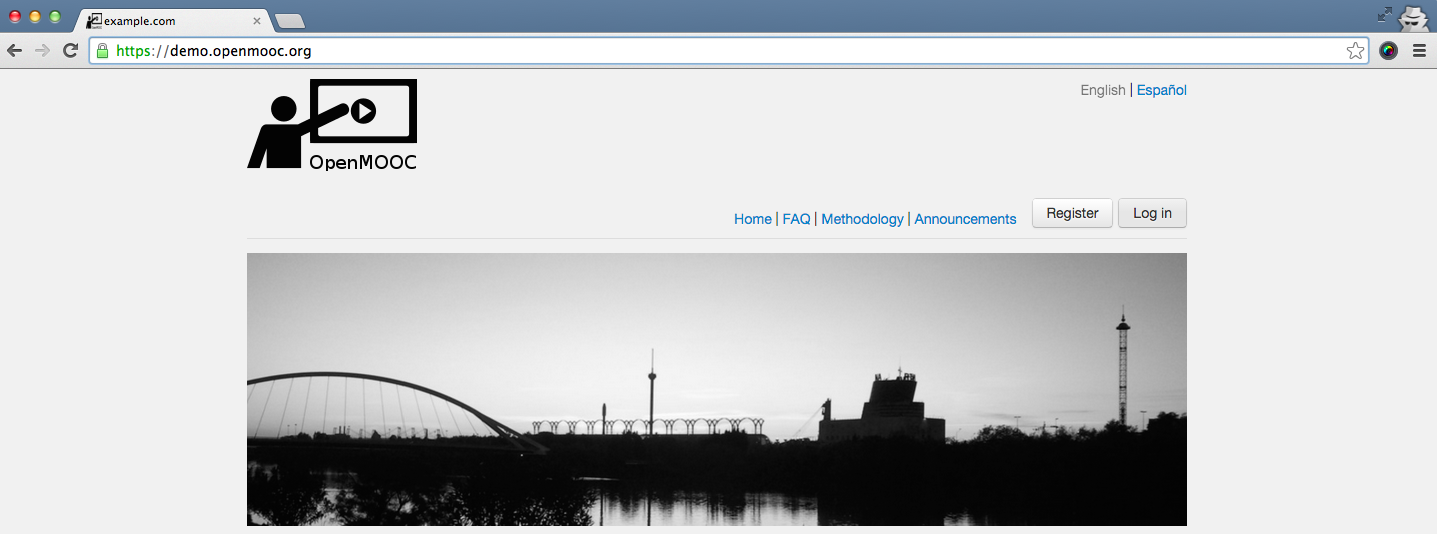
\includegraphics{0_permission_to_create_a_course-1.png}

\item {} 
Fill the \textbf{email} and \textbf{password} fields in the login form.

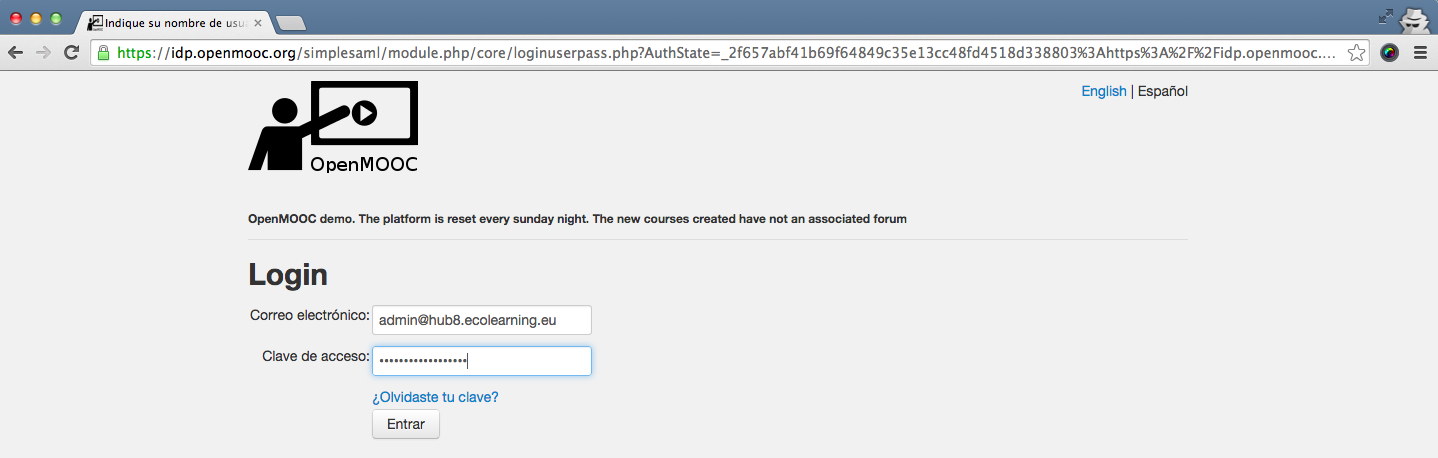
\includegraphics{0_permission_to_create_a_course-2.png}

\item {} 
When you are already logged, selected \textbf{Admin interface} in the dropdown menu you can access by clicking on the user name.

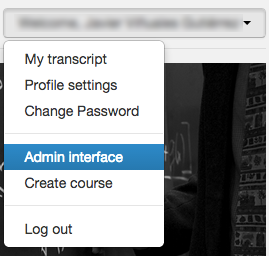
\includegraphics{0_permission_to_create_a_course-3.png}

\item {} 
You have to select \textbf{users} in the admin interface.

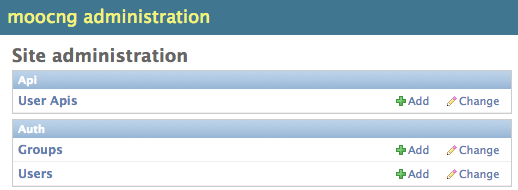
\includegraphics{0_permission_to_create_a_course-4.png}

\item {} 
Enter the name or email of the user you want to give permission to create courses in the search box

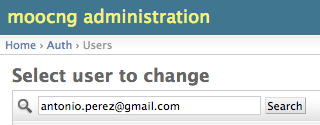
\includegraphics{0_permission_to_create_a_course-5.png}

\item {} 
Select \textbf{Staff status} to give permission to create courses to the user and click \textbf{save} on the bottom of the page.

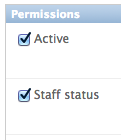
\includegraphics{0_permission_to_create_a_course-6.png}

\end{enumerate}


\chapter{Naming the course}
\label{naming_the_course::doc}\label{naming_the_course:naming-the-course}\label{naming_the_course:id1}

\section{Overview}
\label{naming_the_course:overview}
Only user with permission to crete course can do the following. It's necessary that the administrator
gives permission to create courses to an user, manually on request by email. See


\section{Steps to name a course}
\label{naming_the_course:steps-to-name-a-course}\begin{enumerate}
\item {} 
When you are already logged, selected \textbf{Create course} in the dropdown menu you can access by clicking on the user name.

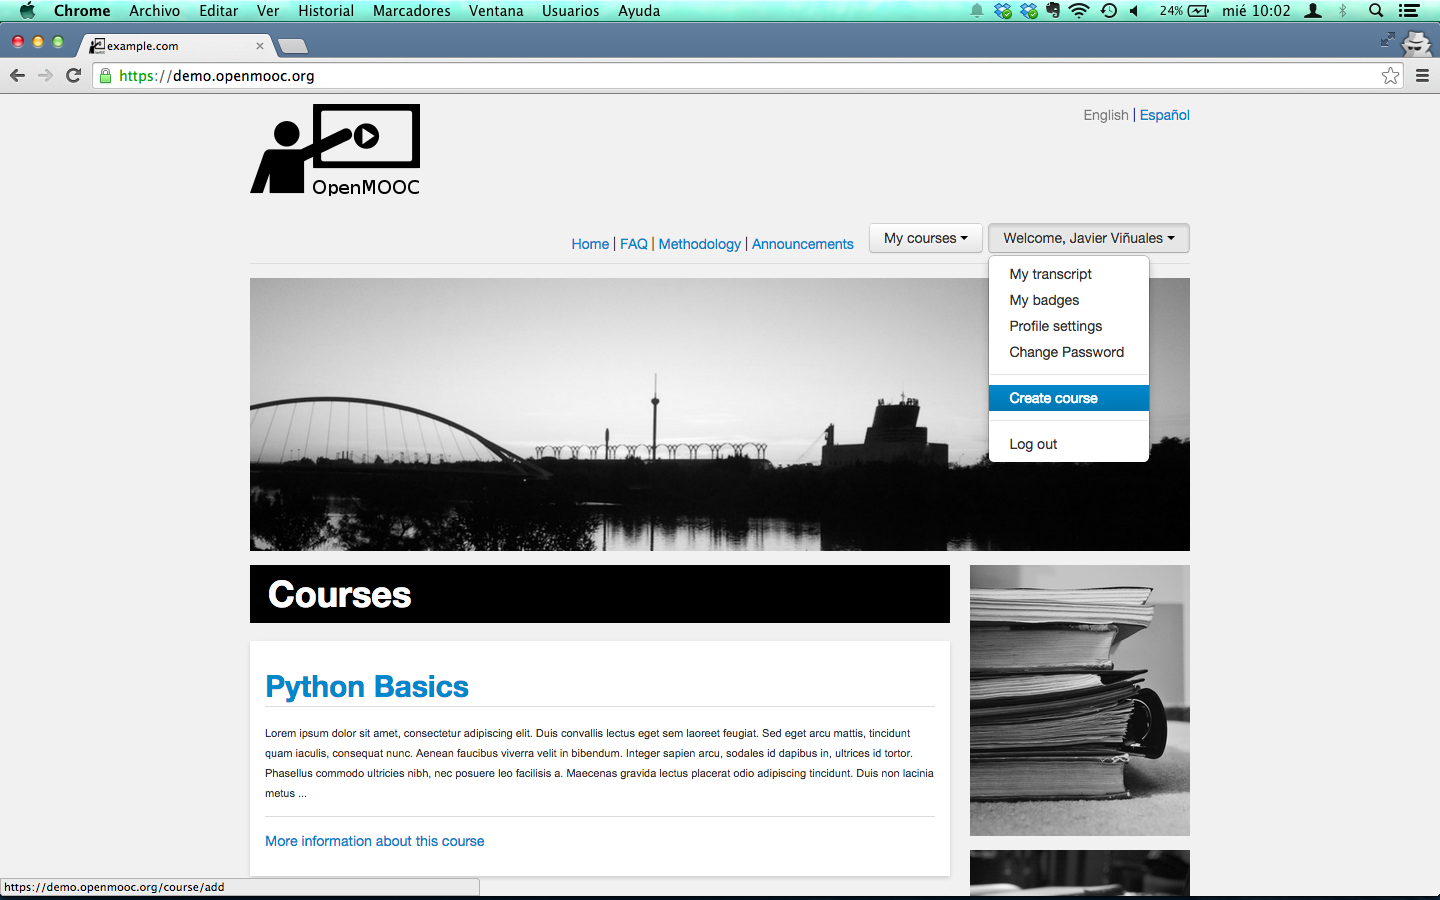
\includegraphics{1_create_course-1.png}

\item {} 
Text box you will se to enter the course name.

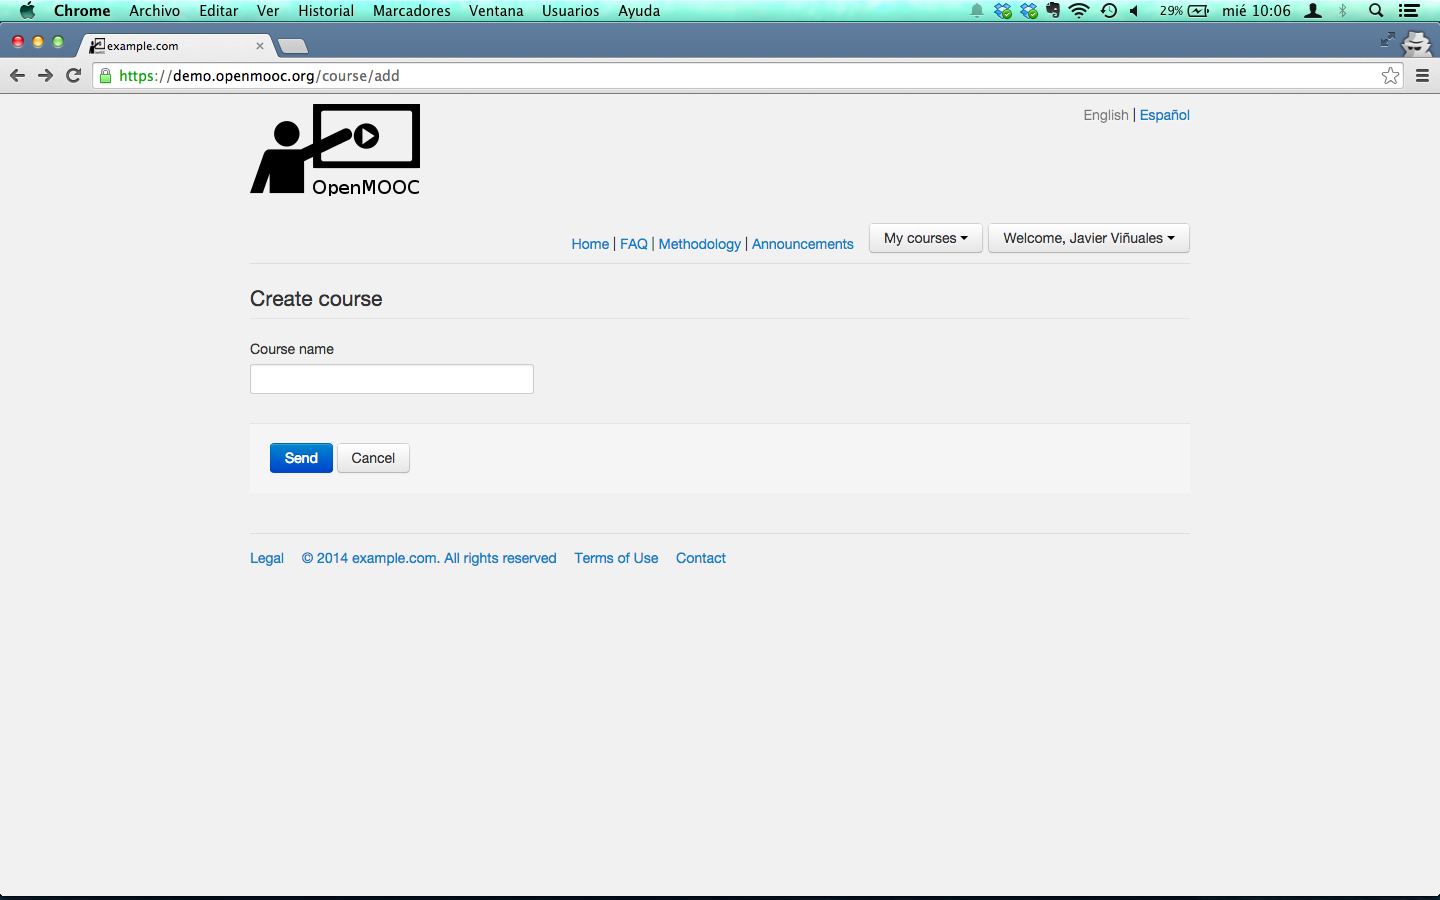
\includegraphics{1_create_course-2.png}

\item {} 
Enter the course name to create courses in the text box and click \textbf{send}.

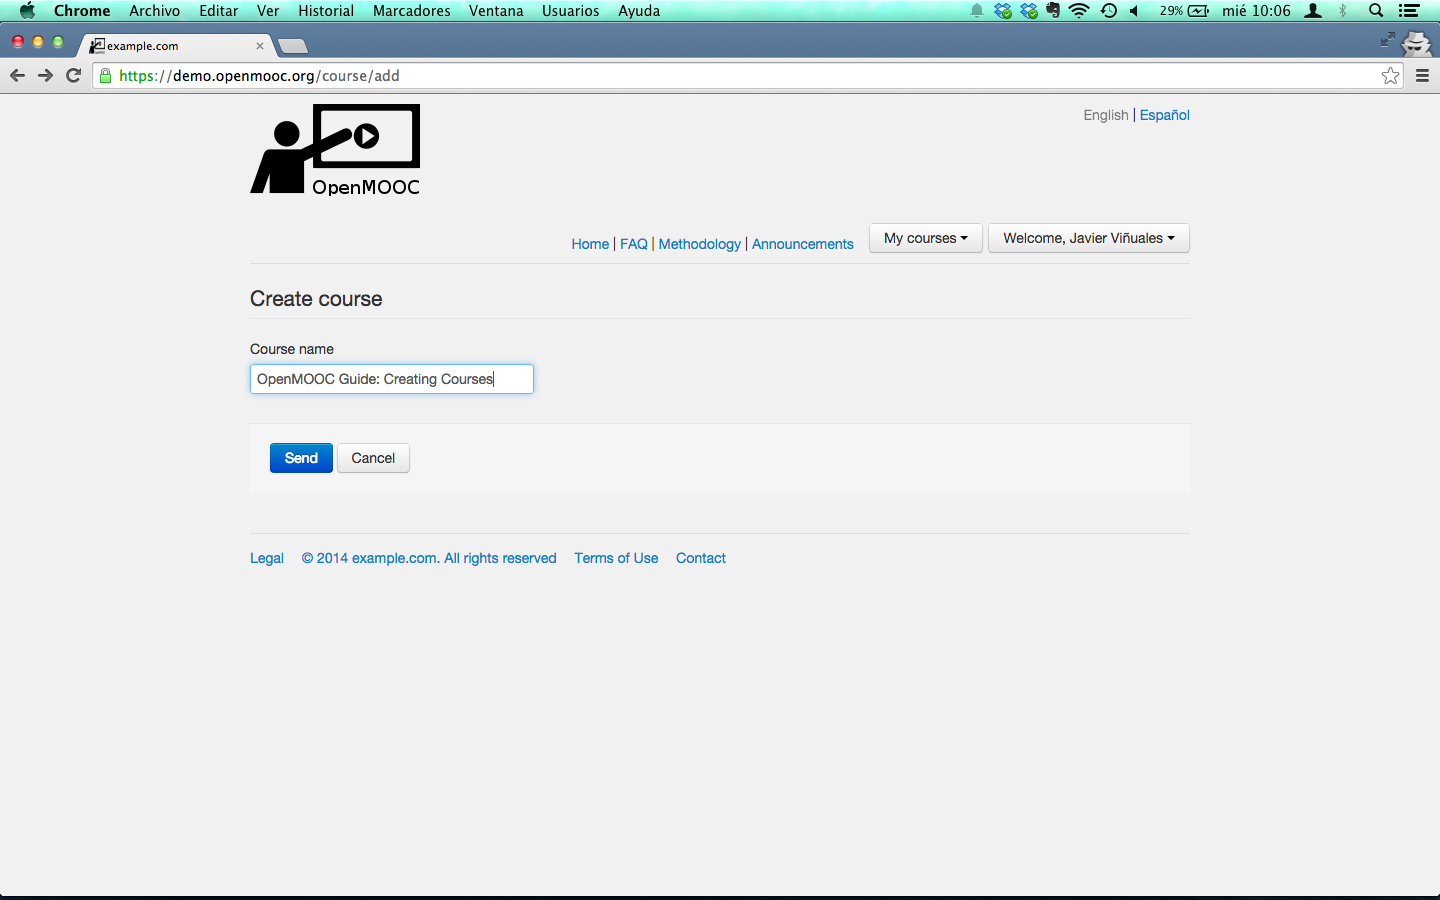
\includegraphics{1_create_course-3.png}

\end{enumerate}


\chapter{The course web page}
\label{course_page:course-page}\label{course_page::doc}\label{course_page:the-course-web-page}

\section{Overview}
\label{course_page:overview}
\begin{notice}{note}{Note:}
You must think about the course web page like the course's landing page.
\end{notice}

At this web page, potential students will reach through the use of search engines or through
other websites where you announce the course. It is important to present the information about the course in a clear and attractive way.

The URL of the course web is optimized for search engines:

\code{https://demo.openmooc.org/course/openmooc-guide-creating-courses/}

This is the appearance of the course web page:
\begin{quote}

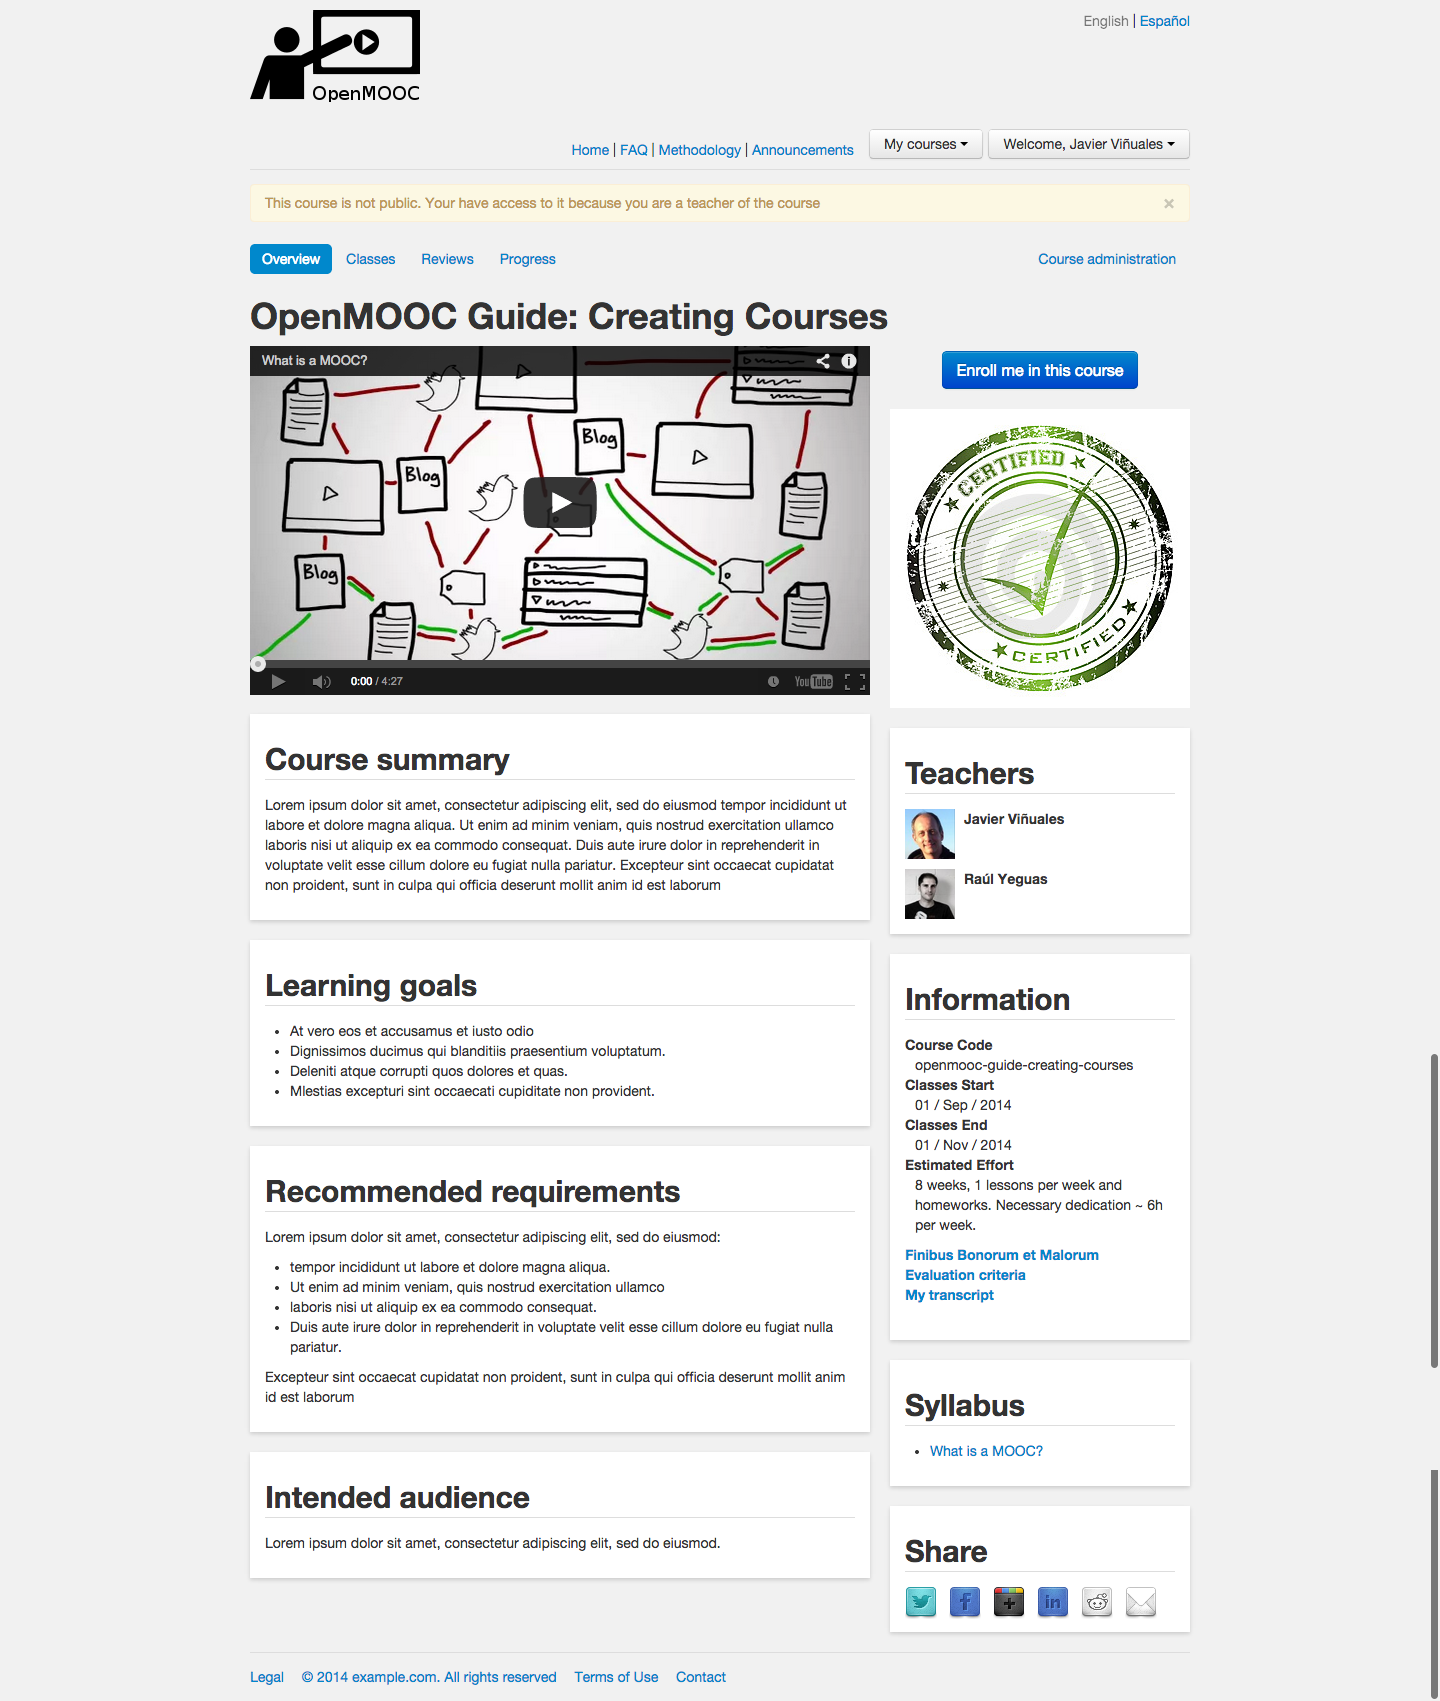
\includegraphics{7_course_view-1.png}
\end{quote}

\begin{notice}{important}{Important:}
To assure that your fill the information in the text boxes \textbf{Description},
\textbf{Requirements}, \textbf{Intended audience}, \textbf{Estimated effort} and \textbf{Learning goals}.
\end{notice}


\section{Accessing to the editing course tool}
\label{course_page:accessing-to-the-editing-course-tool}
When you are already logged, you havet to go the course web page and then, click on the \textbf{Course administration} link.
\begin{quote}

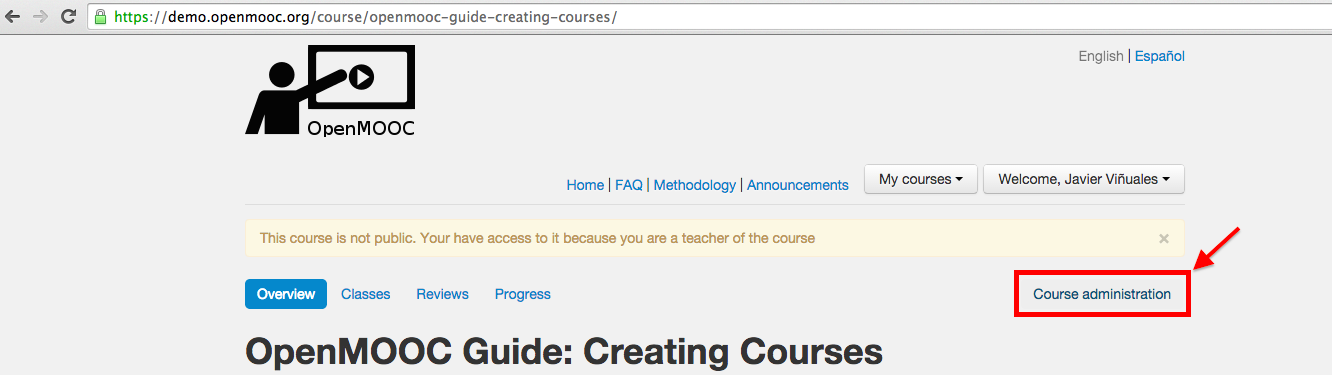
\includegraphics{2_course_information-0.png}
\end{quote}

You will go to the OpenMOOC's course edition tool. The first thing you see is editing course information, which is what forms the course web page.
\begin{quote}

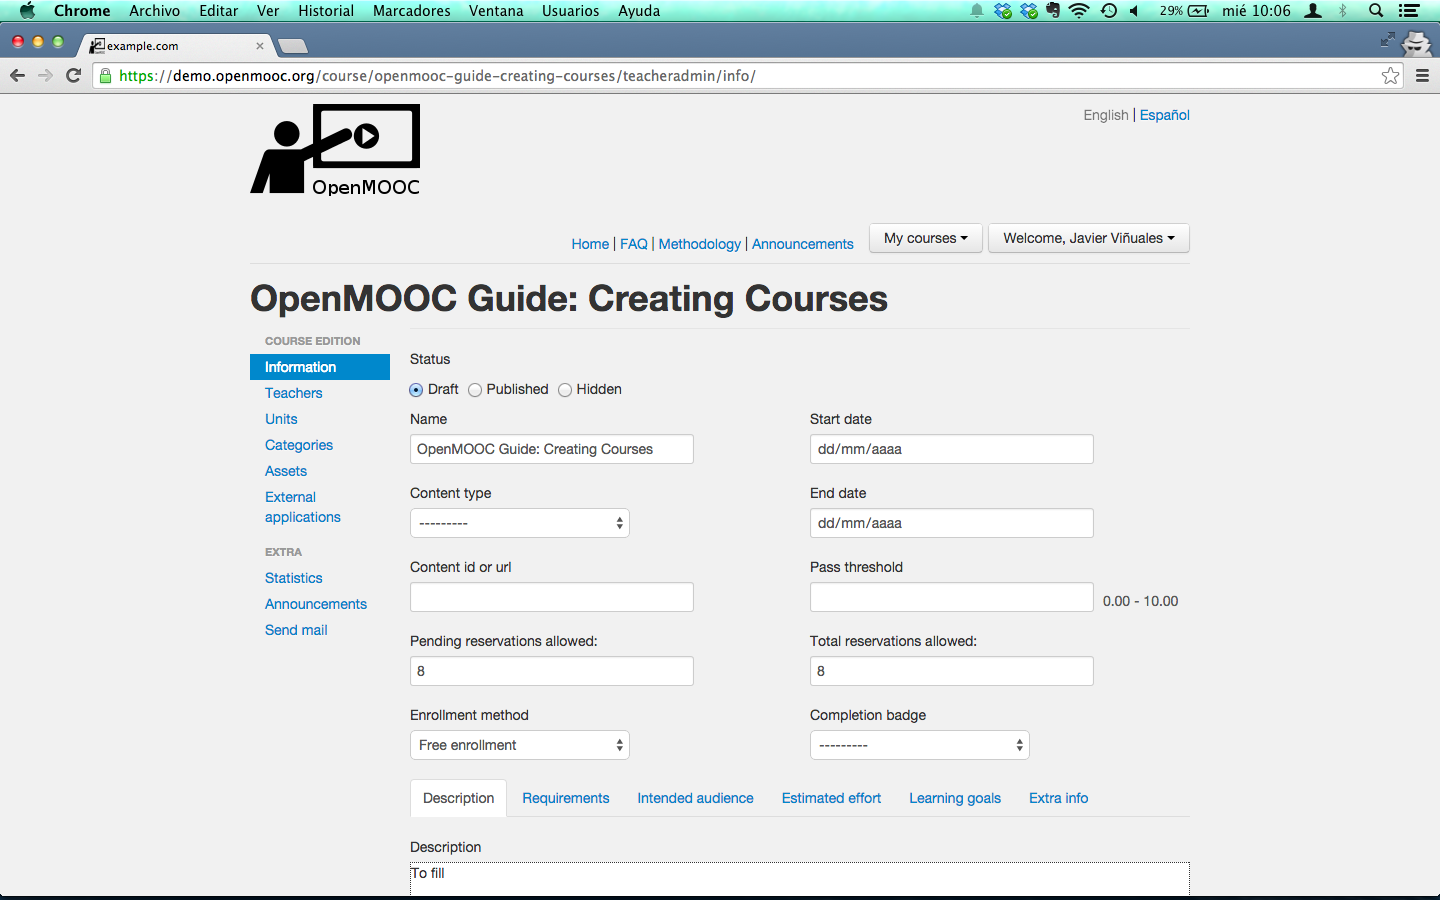
\includegraphics{2_course_information-1.png}
\end{quote}

\begin{notice}{note}{Note:}
The course will always be created in \textbf{draft} state. In the current
draft status is listed in the list of courses available but only viewable by
the course teachers and administrators of the platform. If the course is in \textbf{hidden} state,
it will not appear on the list. If you pass the course to \textbf{published} status, everyone can
see it on the list and enroll.
\end{notice}


\section{Adding the video intro to the course}
\label{course_page:adding-the-video-intro-to-the-course}
You must select an online video source to insert it in the course web page like an intro to the course. OpenMOOC needs the URL of the video and actually supports Youtube, Vimeo, Scribd and Prezi.
\begin{quote}

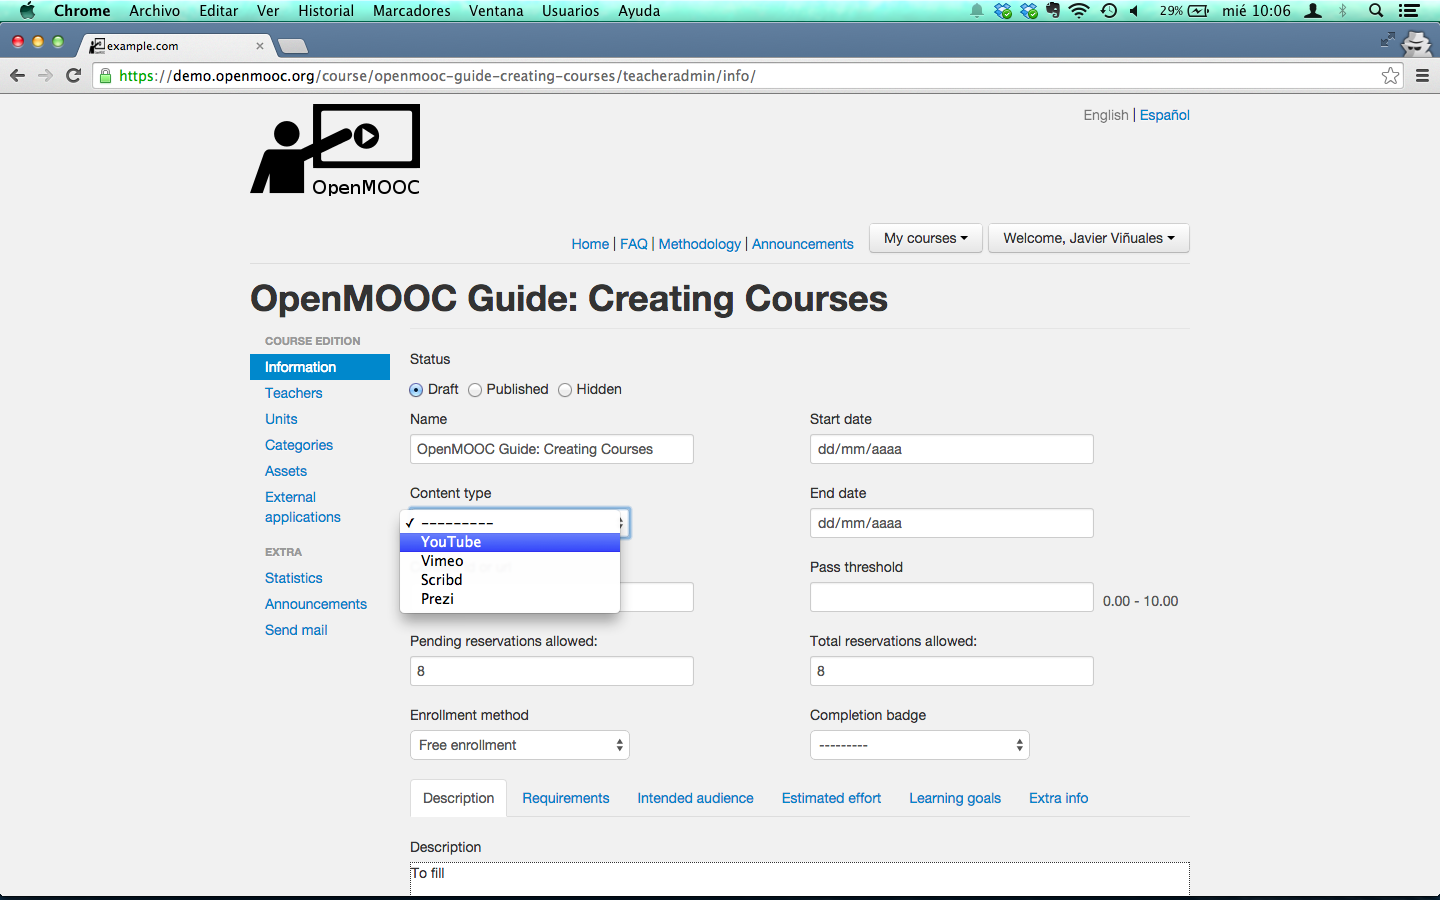
\includegraphics{2_course_information-2a.png}
\end{quote}

Now you can choose a video from Youtube, copy the URL and...
\begin{quote}

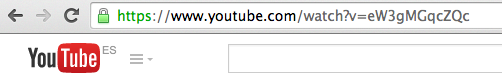
\includegraphics{2_course_information-2b.png}
\end{quote}

...paste it into the text box in the course edition tool.
\begin{quote}

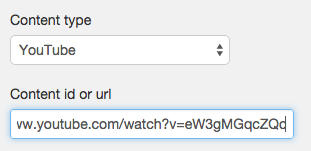
\includegraphics{2_course_information-2c.png}
\end{quote}

\begin{notice}{note}{Note:}
We recommend the use of a Youtube Channel for each organization and then,
the use of playlists to group videos for each course. You can use channels on Vimeo too,
and albums to group videos for each course.
\end{notice}


\section{Setting the start date and end date of the course}
\label{course_page:setting-the-start-date-and-end-date-of-the-course}
You can enter the start date by hand into the text box or choose it from the calendar view.
\begin{quote}

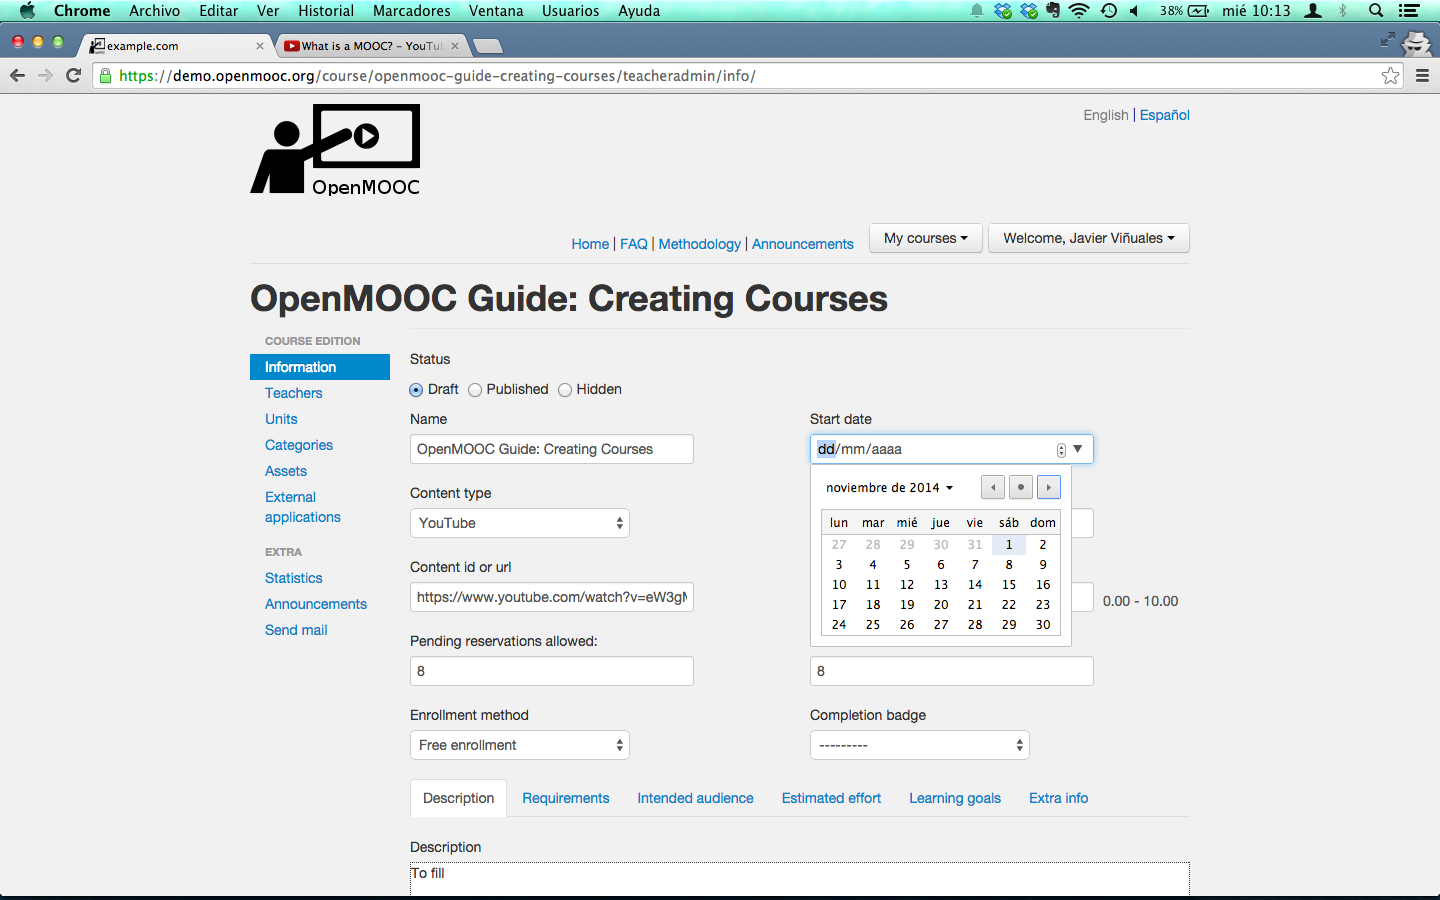
\includegraphics{2_course_information-3.png}
\end{quote}

Do the same to enter the end date of the course.
\begin{quote}

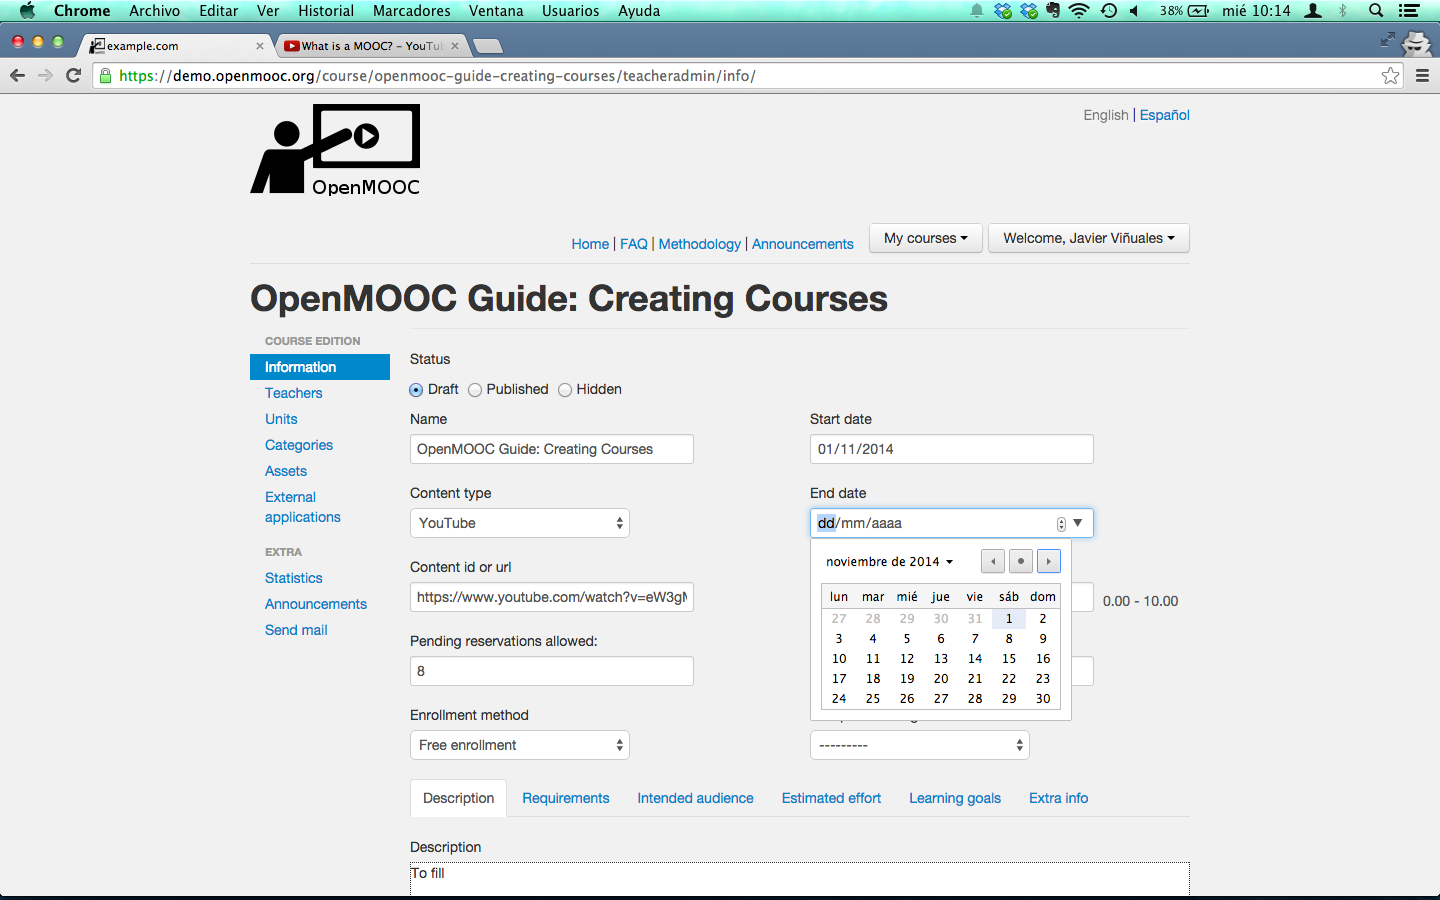
\includegraphics{2_course_information-4.png}
\end{quote}

\begin{notice}{important}{Important:}
Before the start date and being in published state, anyone can enroll.
After the end date, the course will be closed.
\end{notice}


\section{Setting the threshold to pass the course}
\label{course_page:setting-the-threshold-to-pass-the-course}
You must fix the threshold to pass the course. If a student's grade in the course exceeds the threshold, are
deemed to have accepted the course, and if you created a certificate for the course, the student may obtain it.
\begin{quote}

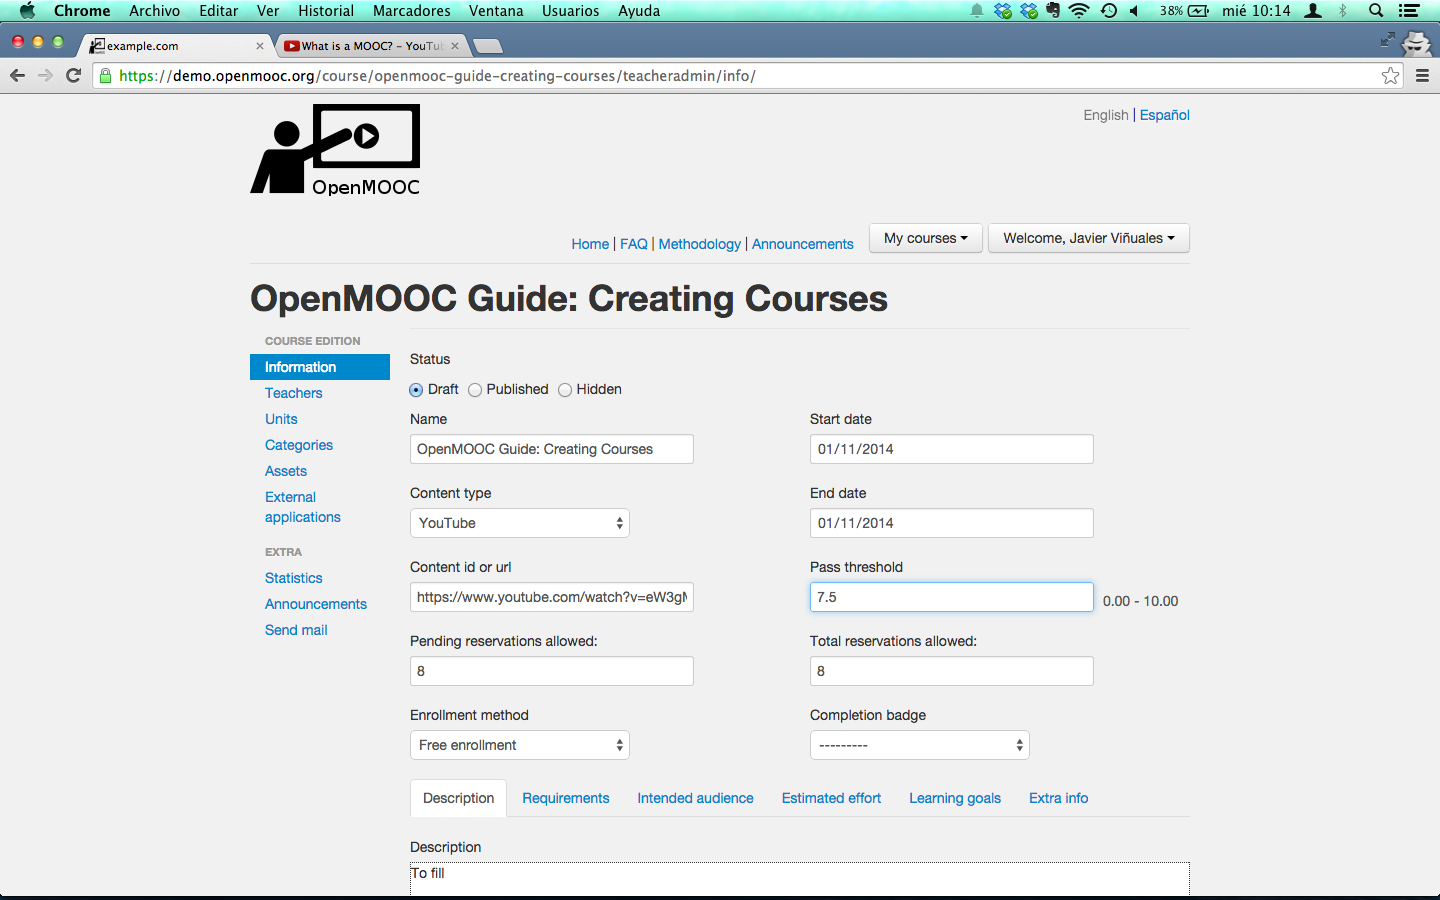
\includegraphics{2_course_information-5.png}
\end{quote}


\section{Writing the description of the course}
\label{course_page:writing-the-description-of-the-course}
The description of the course is formed by the contents of the tabs \textbf{Description}, \textbf{Requirements},
\textbf{Intended audience}, \textbf{Estimated effort} and \textbf{Learning goals}. It's very important not leave empty
the contents of the previous tabs. An additional tab named \textbf{Extra info} is optional.

Fill \textbf{Description} text area.
\begin{quote}

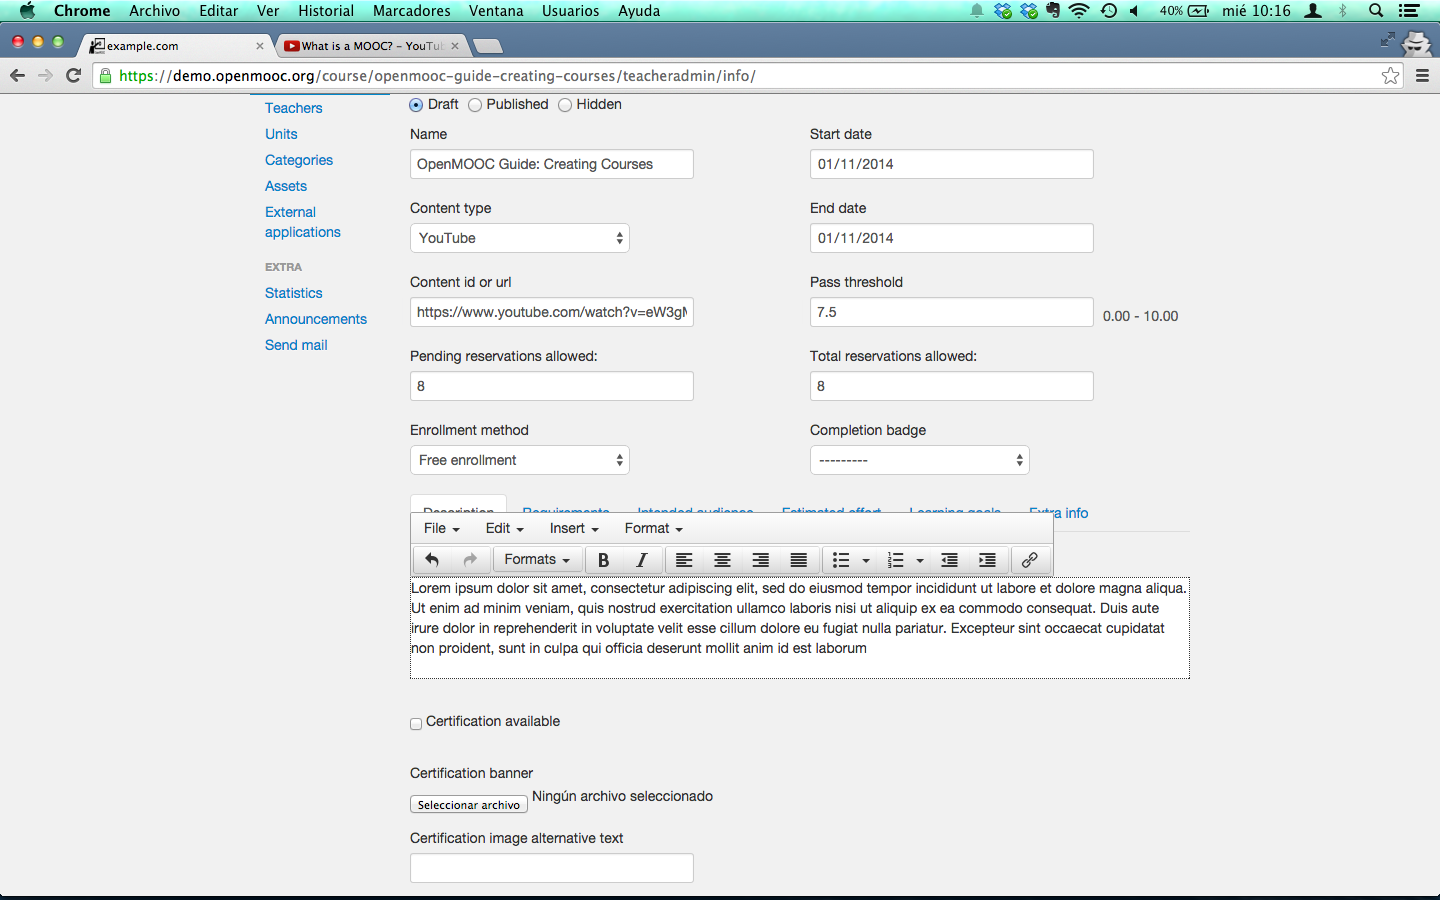
\includegraphics{2_course_information-6.png}
\end{quote}

Fill \textbf{Requirements} text area.
\begin{quote}

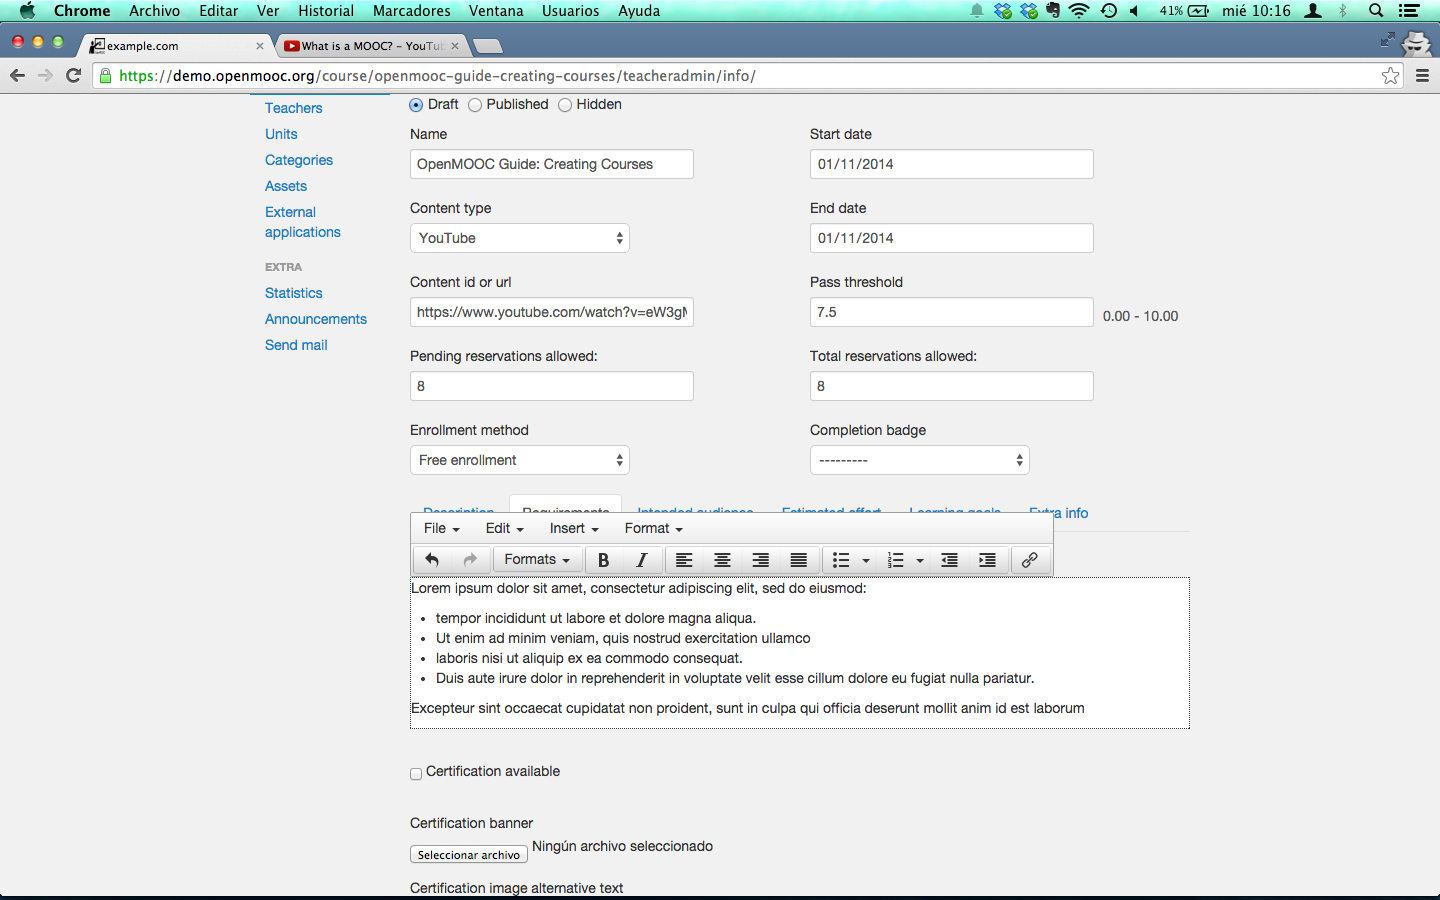
\includegraphics{2_course_information-7.png}
\end{quote}

Fill \textbf{Intended audience} text area.
\begin{quote}

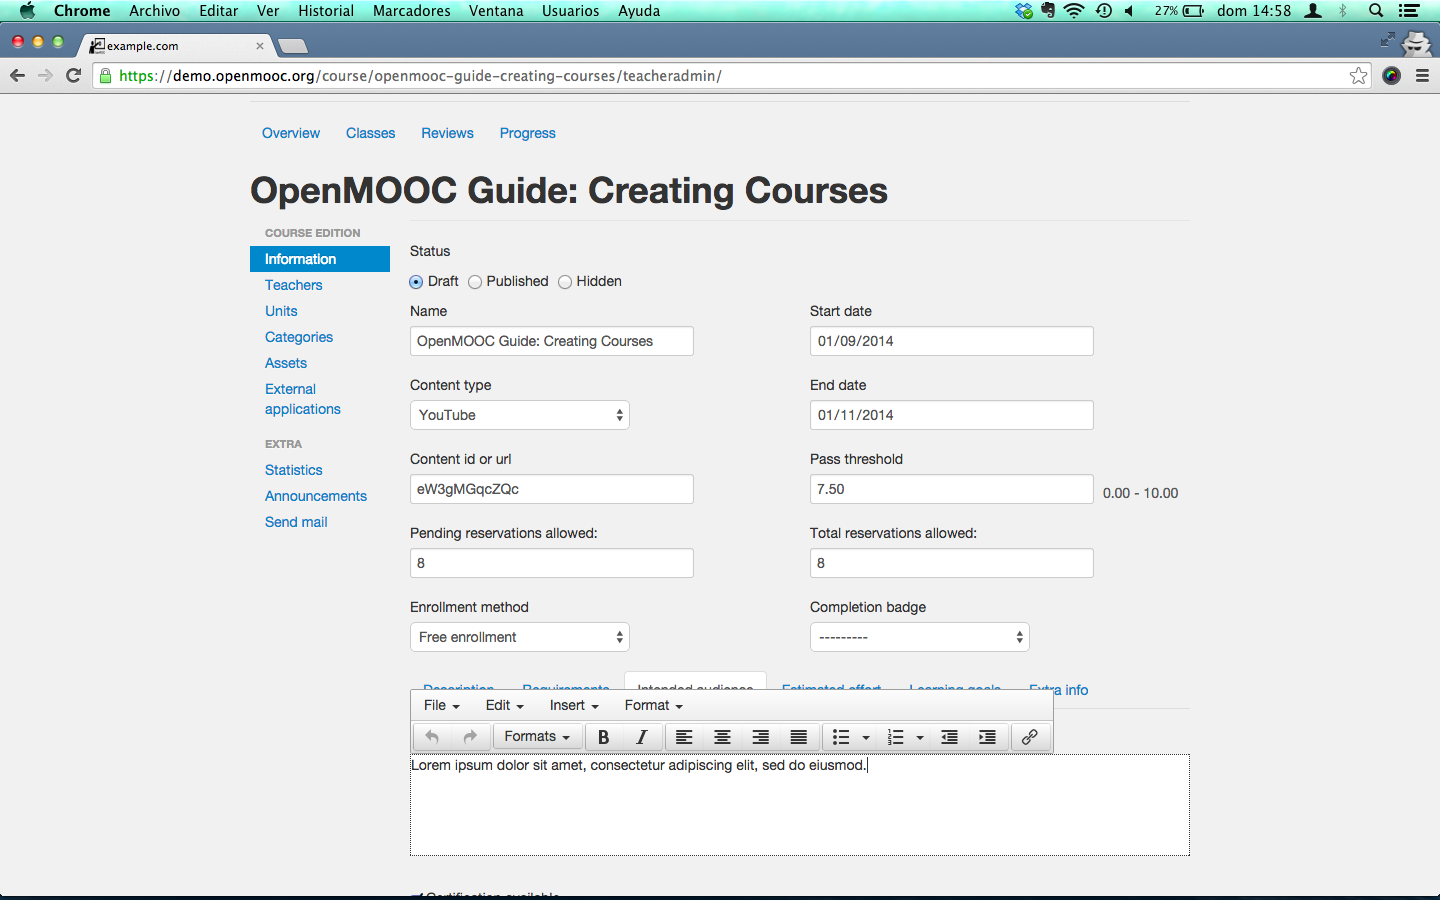
\includegraphics{2_course_information-8.png}
\end{quote}

Fill \textbf{Estimated effort} text area.
\begin{quote}

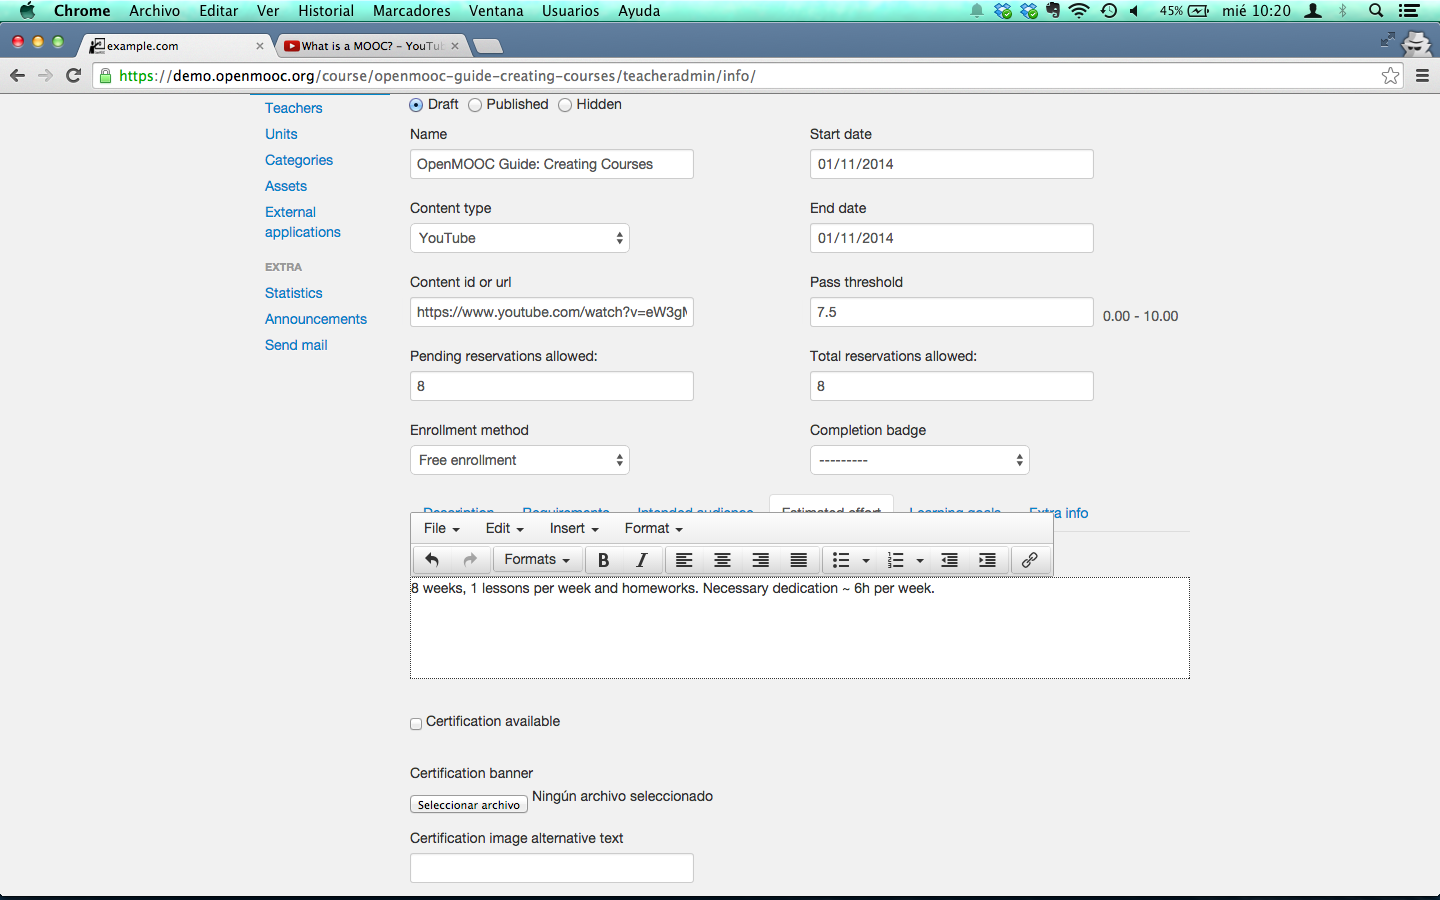
\includegraphics{2_course_information-9.png}
\end{quote}

Fill \textbf{Learning goals} text area.
\begin{quote}

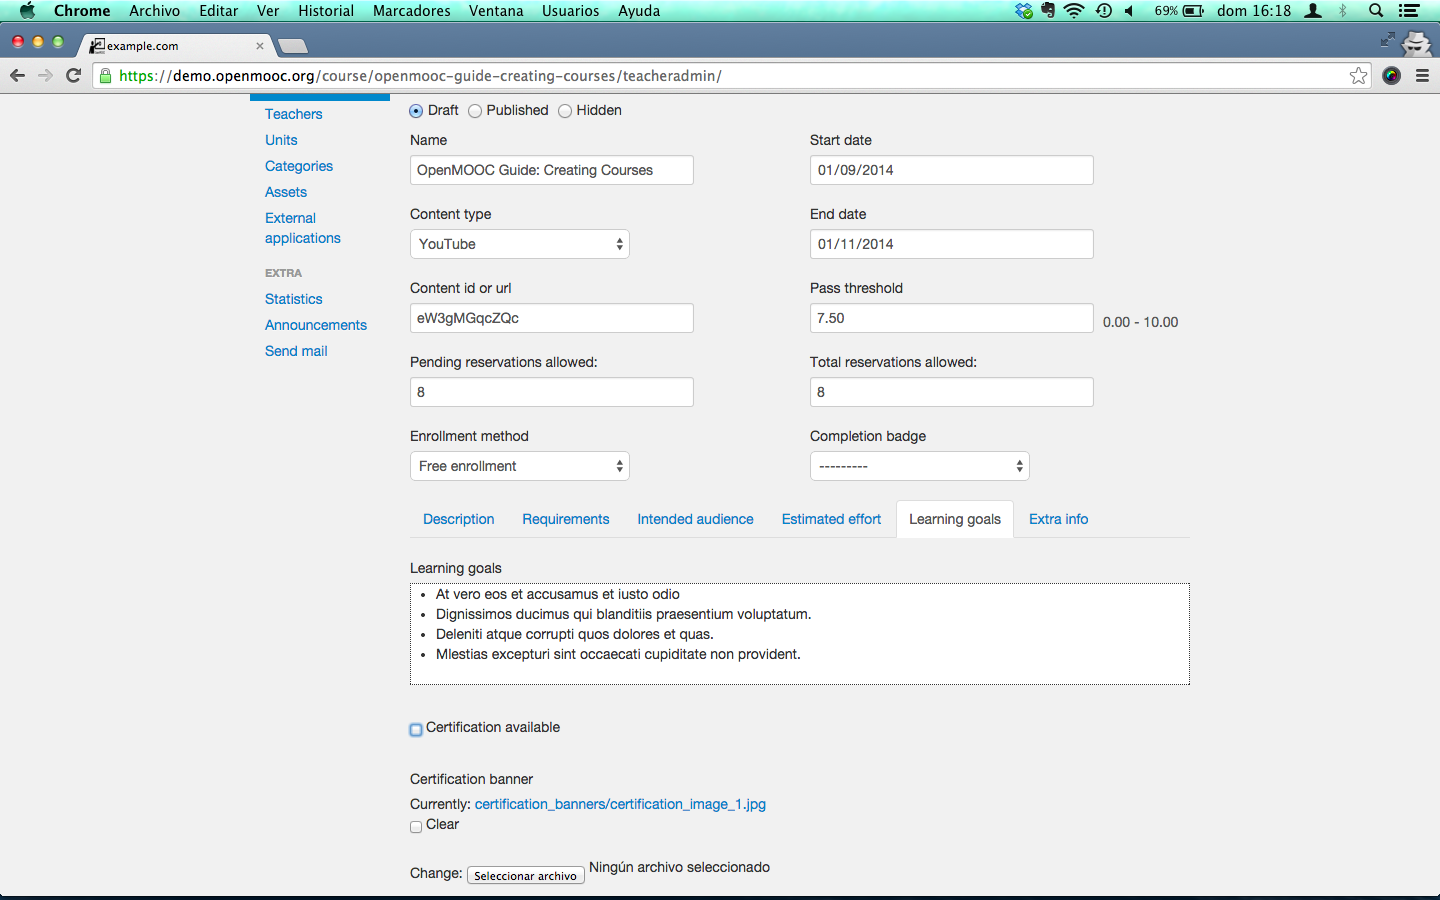
\includegraphics{2_course_information-10.png}
\end{quote}

Optionally, fill \textbf{Extra info} text area.
\begin{quote}

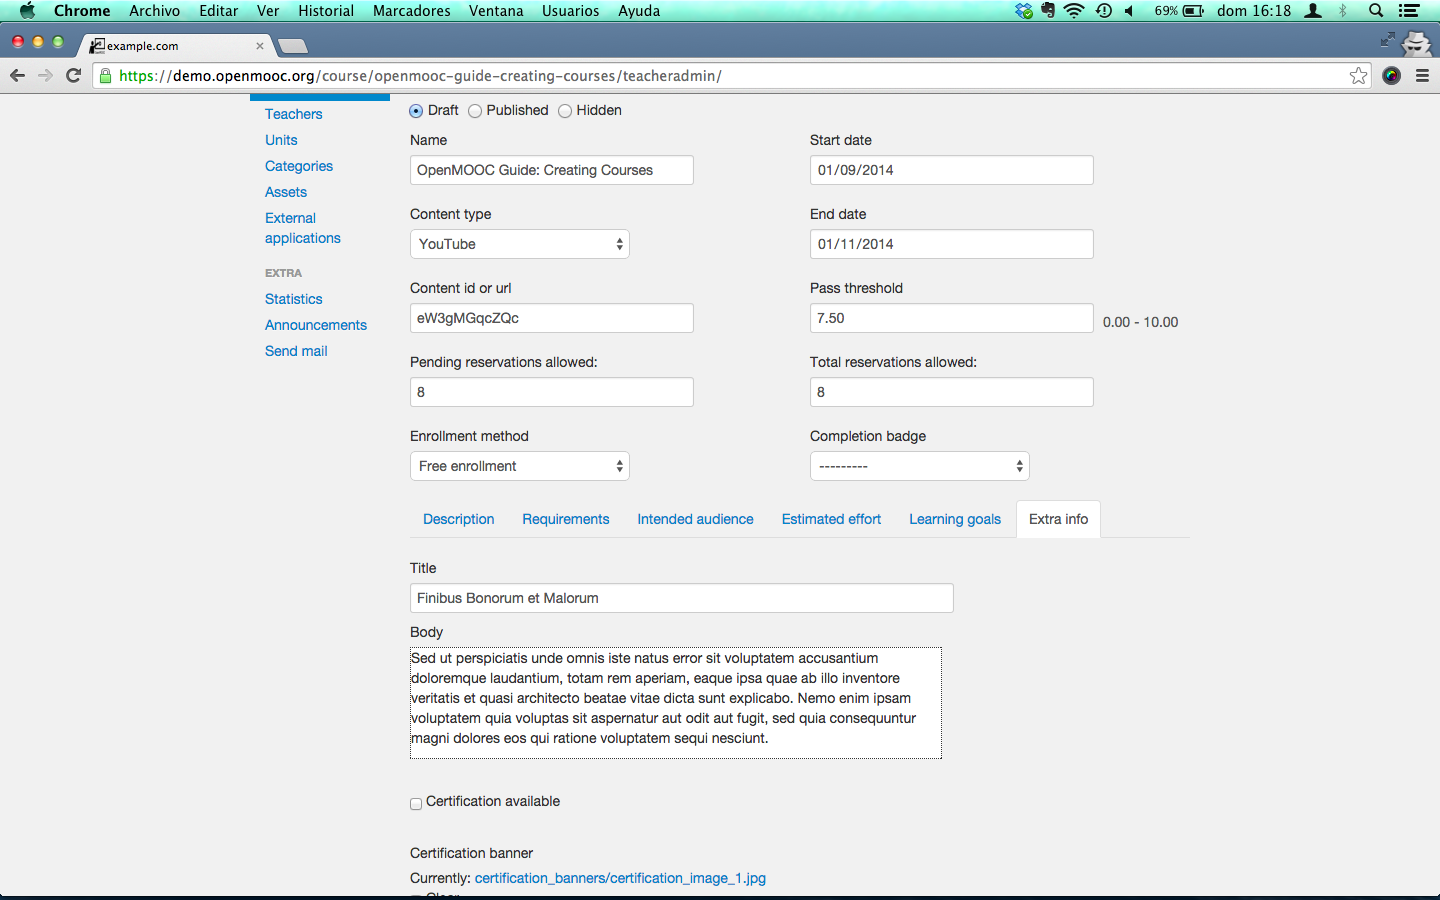
\includegraphics{2_course_information-11.png}
\end{quote}


\section{Associating a certificate to the course}
\label{course_page:associating-a-certificate-to-the-course}
You must select the \textbf{Certification available} check box and choose a file to
use like the certification's logo. You can select the logo file from your file system.
\begin{quote}

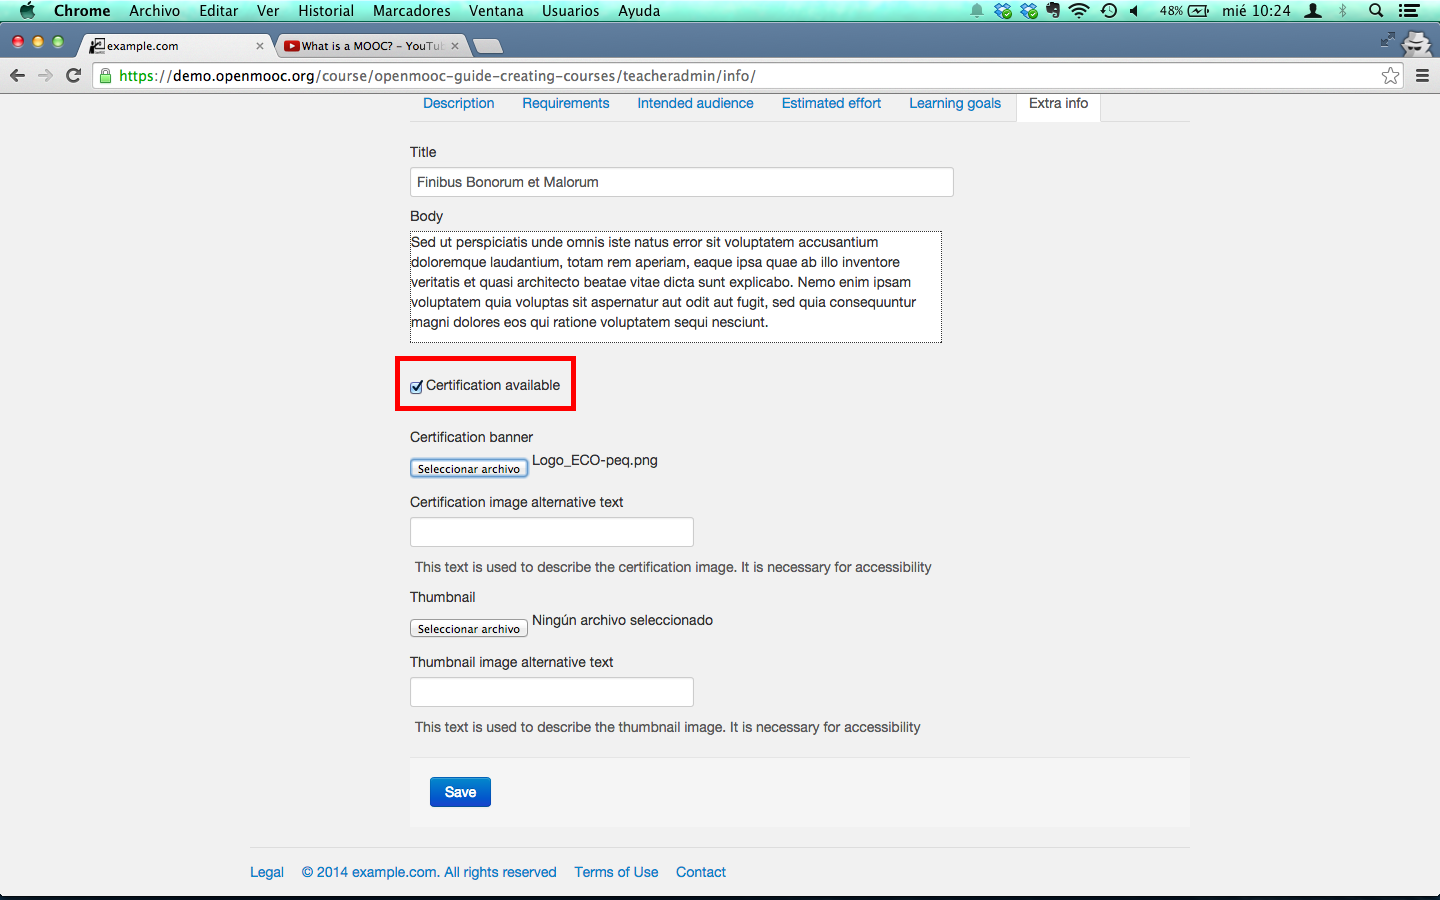
\includegraphics{2_course_information-12.png}
\end{quote}

The last thing you have to do is add an alternative text to the image of the
certification, and click on the \textbf{Save} button you can find in the bottom of
the course web.
\begin{quote}

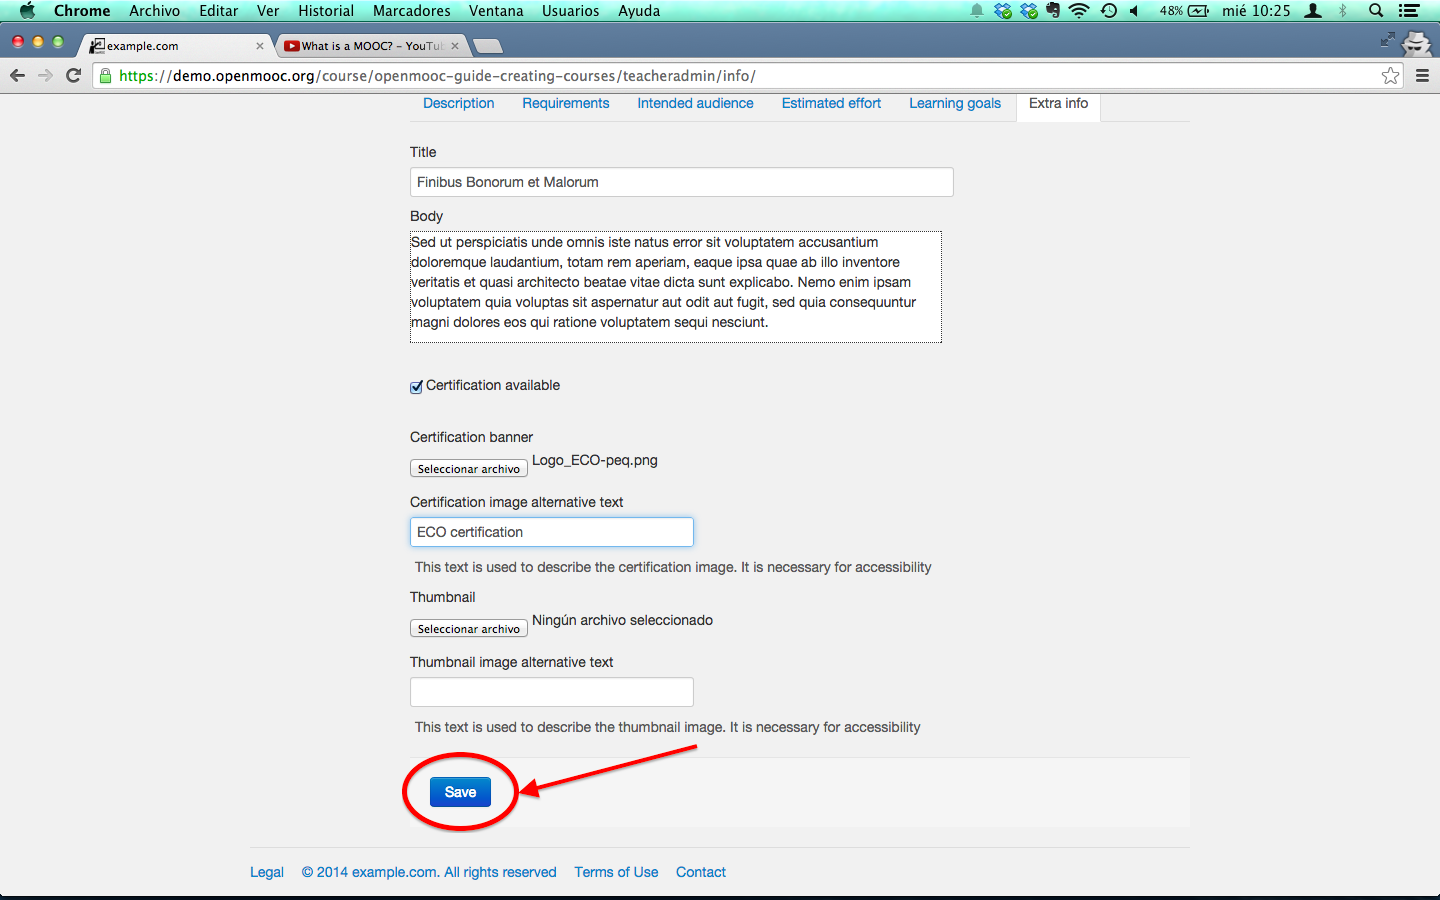
\includegraphics{2_course_information-13.png}
\end{quote}


\chapter{Course teachers}
\label{course_teachers:course-teachers}\label{course_teachers::doc}\label{course_teachers:id1}

\section{Overview}
\label{course_teachers:overview}
The user who creates the course is by default the owner but, he can
transfer the ownership to another course teacher.

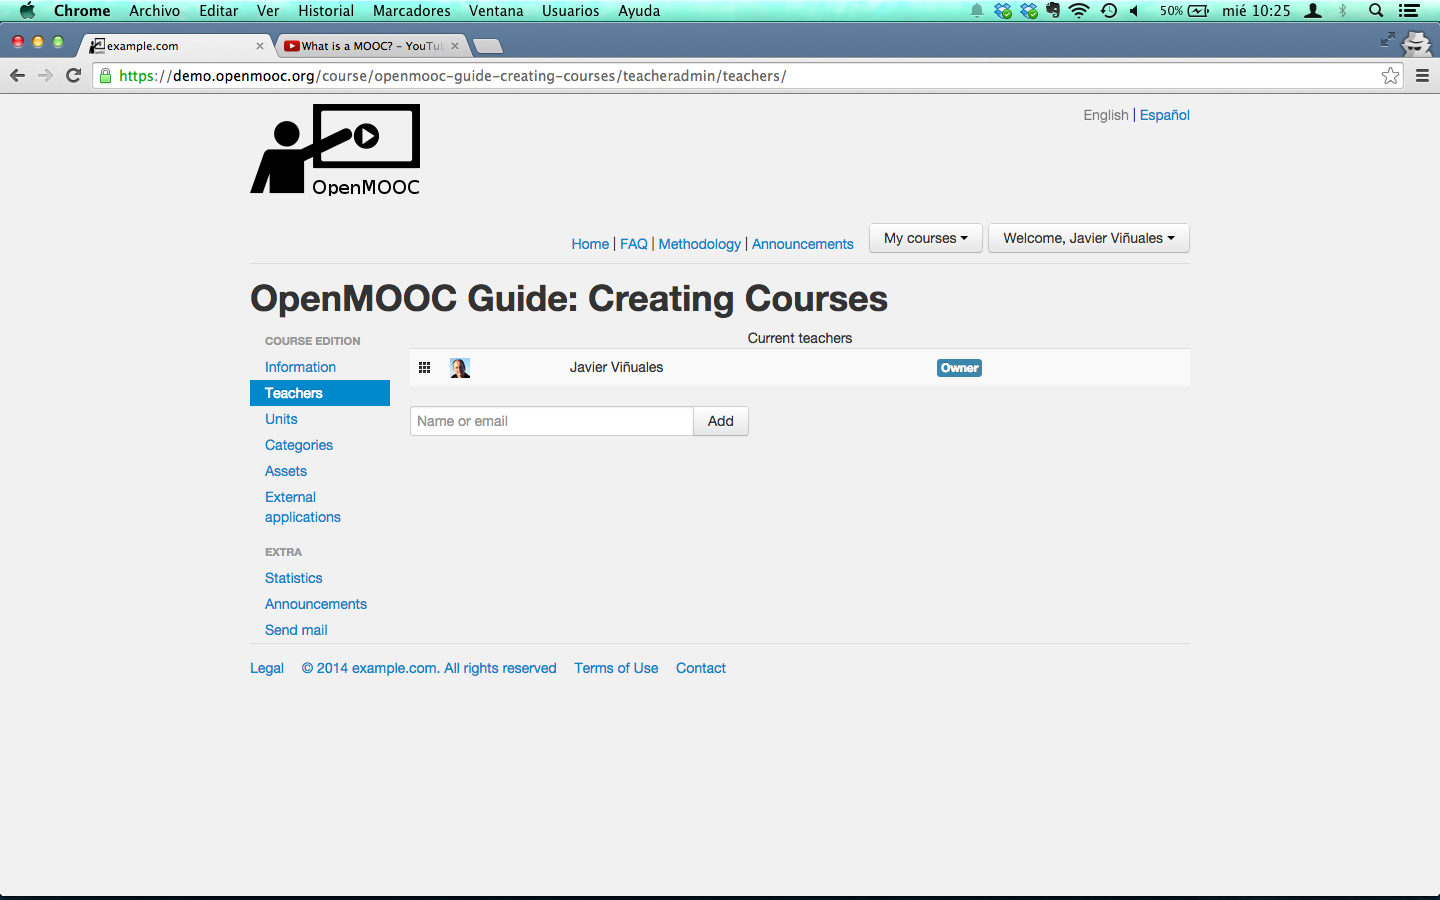
\includegraphics{3_course_teachers-1.png}

The owner user can add additional teachers to the course, forming the
teaching staff of the course.

To add a teacher, can be searched by name or by email and if not yet a user of the platform,
you will be sent an invitation to register. The teacher who is invited to join the team of a
course always receive an email about it.


\section{Steps to add teachers to a course}
\label{course_teachers:steps-to-add-teachers-to-a-course}\begin{enumerate}
\item {} 
Select the user to add like a new teacher of the course.

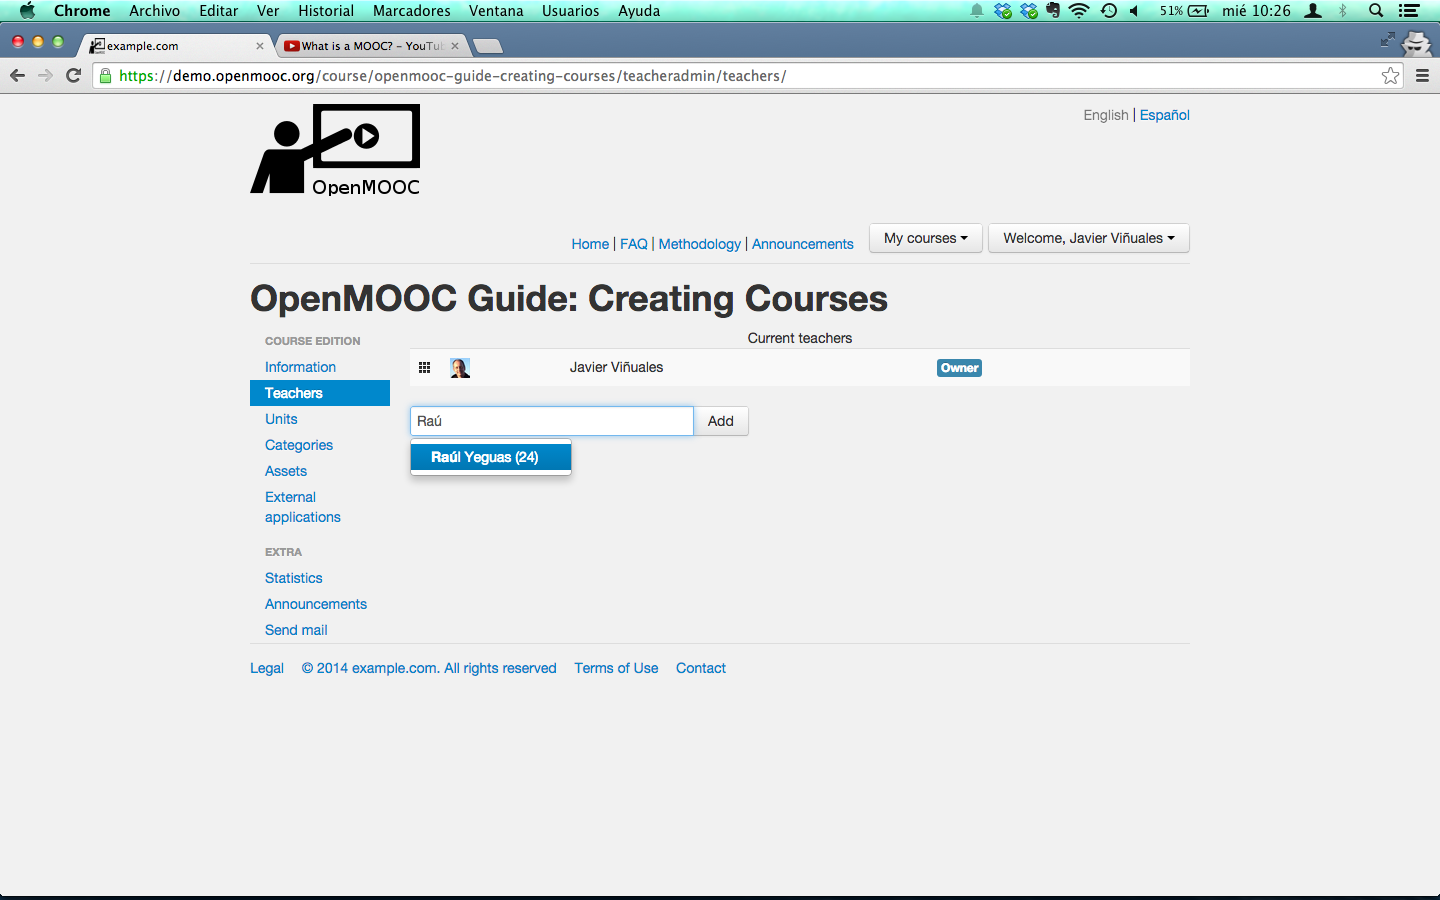
\includegraphics{3_course_teachers-2.png}

\item {} 
The user you added is listed and you get a message from the platform like \code{Success: The teacher has been added to the course or invited}.

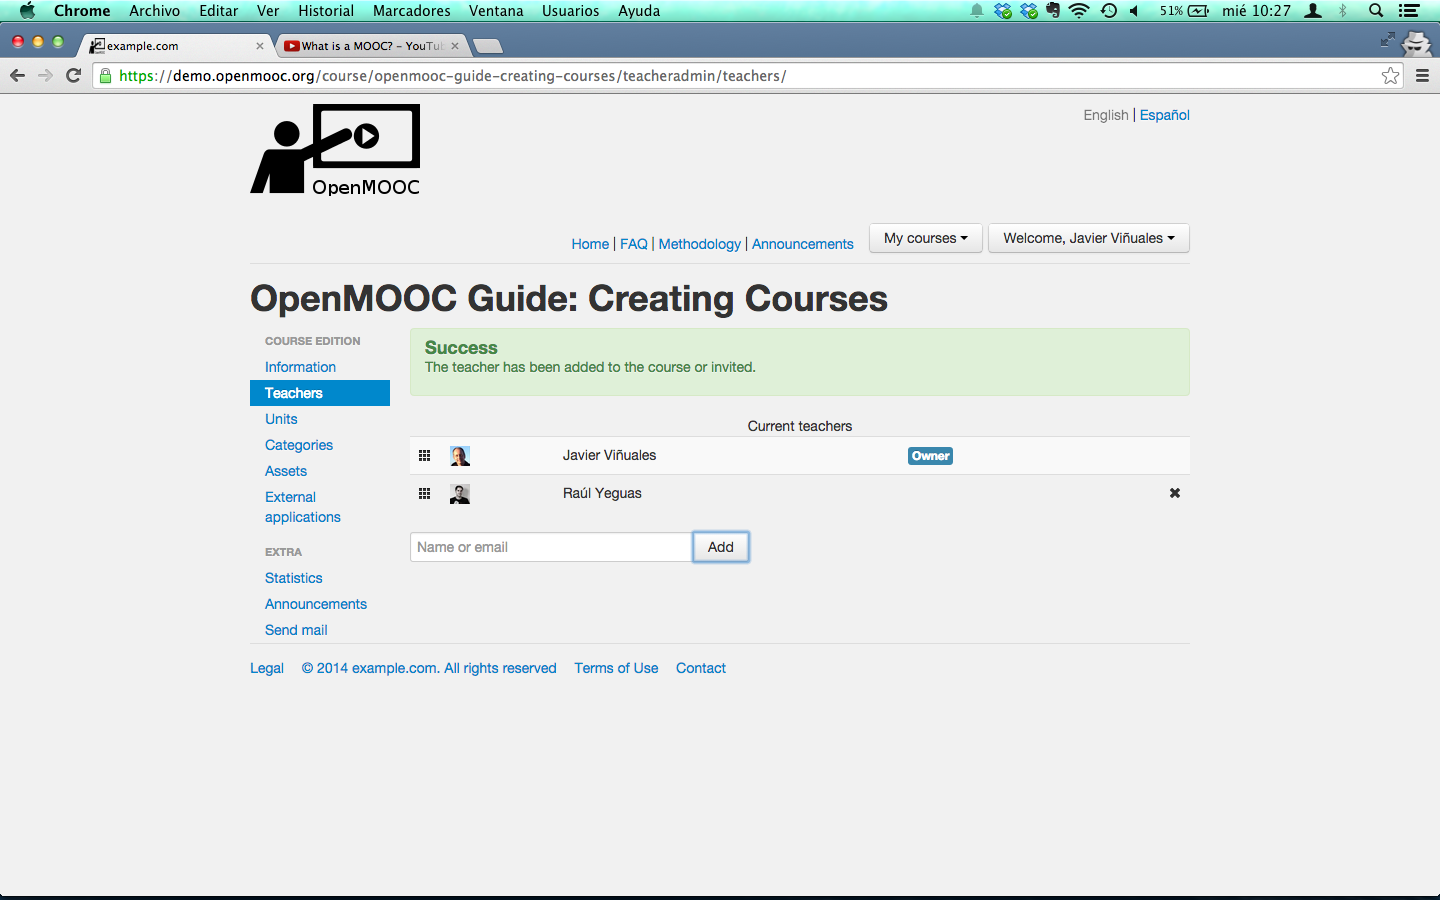
\includegraphics{3_course_teachers-3.png}

\item {} 
If you want to transfer the ownership you can do it new because there are more than one teacher in the course staff.

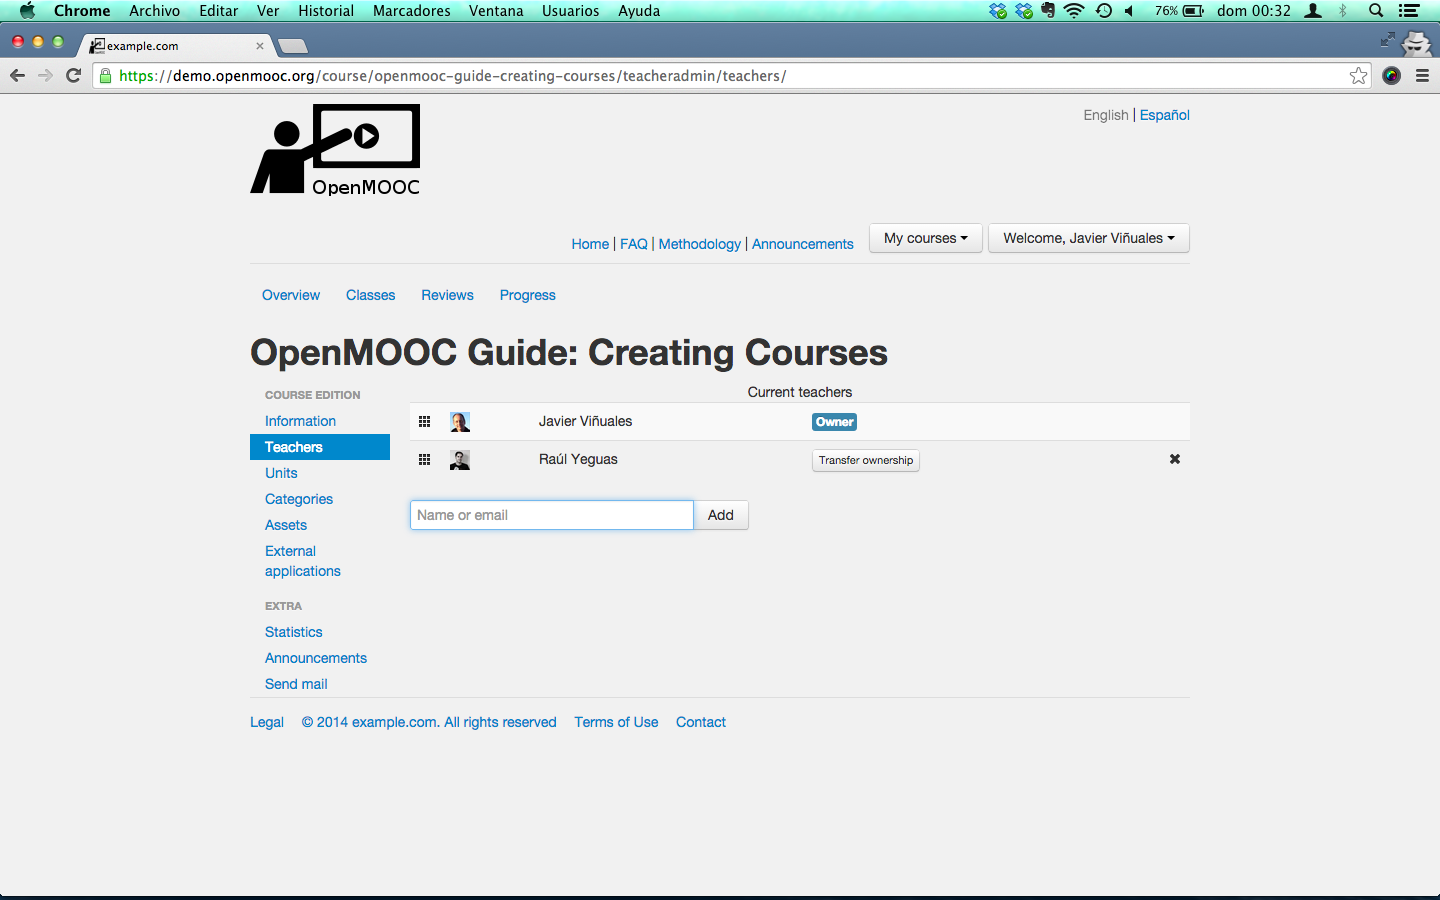
\includegraphics{3_course_teachers-4.png}

\end{enumerate}


\chapter{Course units}
\label{course_units:course-units}\label{course_units::doc}\label{course_units:id1}

\section{Course, units and pills}
\label{course_units:course-units-and-pills}
OpenMOOC have three levels for contents: course, units and pills.


\subsection{Course}
\label{course_units:course}
A \textbf{course} consists of:
\begin{itemize}
\item {} 
General information on the course, teachers.

\item {} 
The units that form.

\end{itemize}


\subsection{Unit}
\label{course_units:unit}
A \textbf{unit} consist of pills and there are three types of units:
\begin{itemize}
\item {} 
Normal, to expose the contents and usually published weekly.

\item {} 
Homework, to promote the individual and groupal work, usually
published weekly and related with the contents exposed in the normal unit of that week.

\item {} 
Exam, to measure the assimilation of content by students.

\end{itemize}

Homework and exam are limited in time, with a start and end time.


\subsection{Pill}
\label{course_units:pill}
A \textbf{pill} consist of:
\begin{itemize}
\item {} 
One online video from Youtube or Vimeo (or prezi or scribd content) like central content.

\item {} 
Comments by the teacher to clarify some thing exposed in the video.

\item {} 
Additional material to extend the content exposed in the video.

\item {} 
Some file attached.

\end{itemize}

You can add forms or peer review tasks to a pill.

\begin{notice}{note}{Note:}
The optimal use is adding some questions to normal units (not in all the pills) and
not use peer review. It's better the use of peer review in homework units.
\end{notice}


\section{Creating the course structure}
\label{course_units:creating-the-course-structure}
When you know the three levels of content with which OpenMOOC works, you can create the course structure.
To create the structure you need to click on \textbf{Units}.
\begin{enumerate}
\item {} 
You will get a message like \code{This course is empty: You need to add content to this course. Please, start adding an unit}.

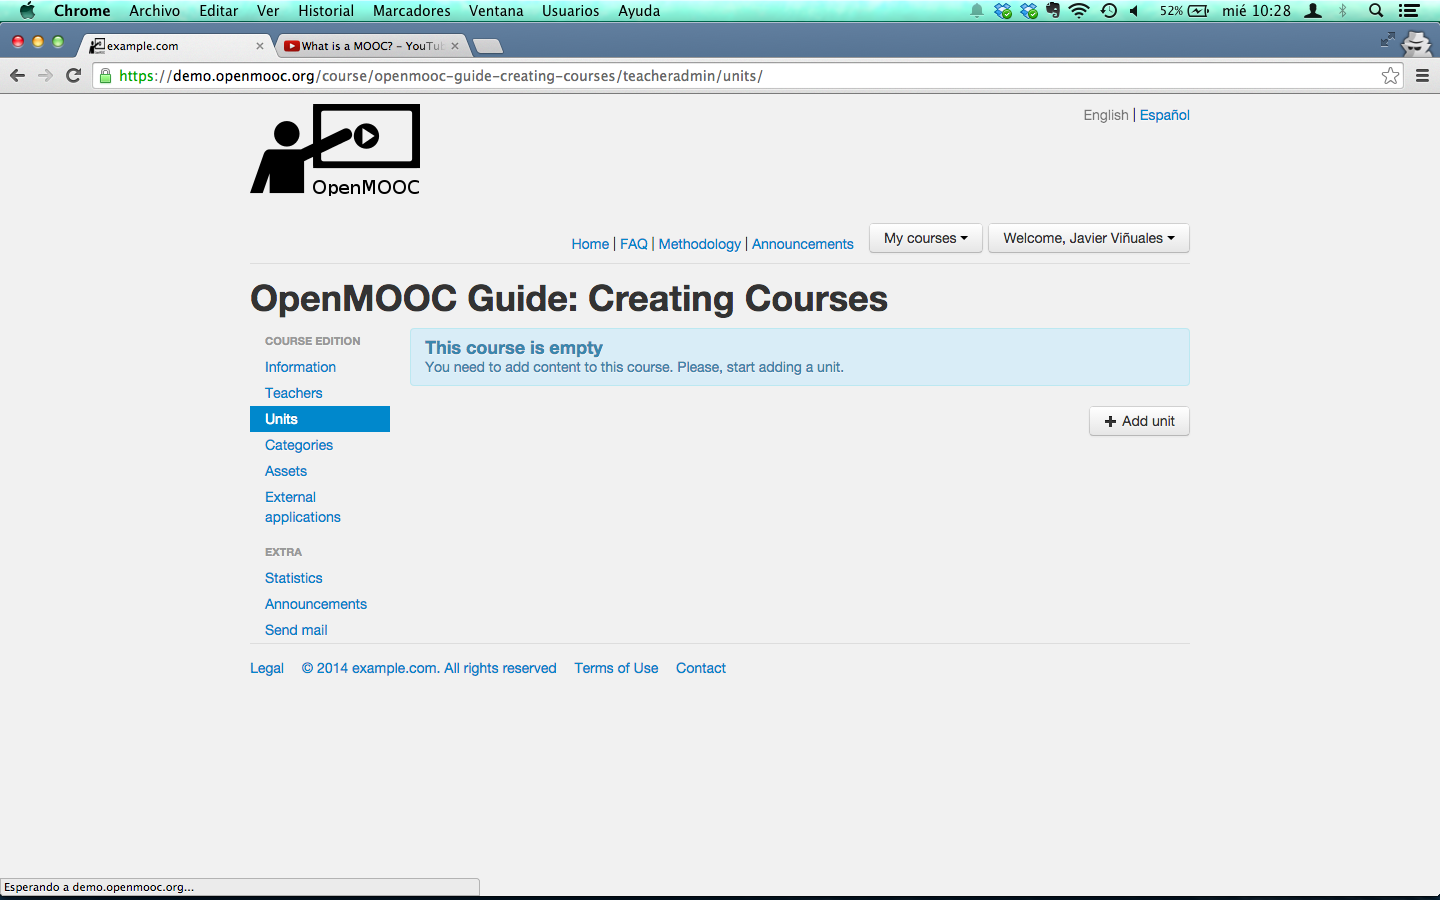
\includegraphics{4_course_units-1.png}

\item {} 
Click on \textbf{Add unit} button and you will get a form. You have to fill the name of the Unit, the type (Normal, Homework or Exam) and a weight. We recommend leaving the weights for the end, when you have done the entire course.

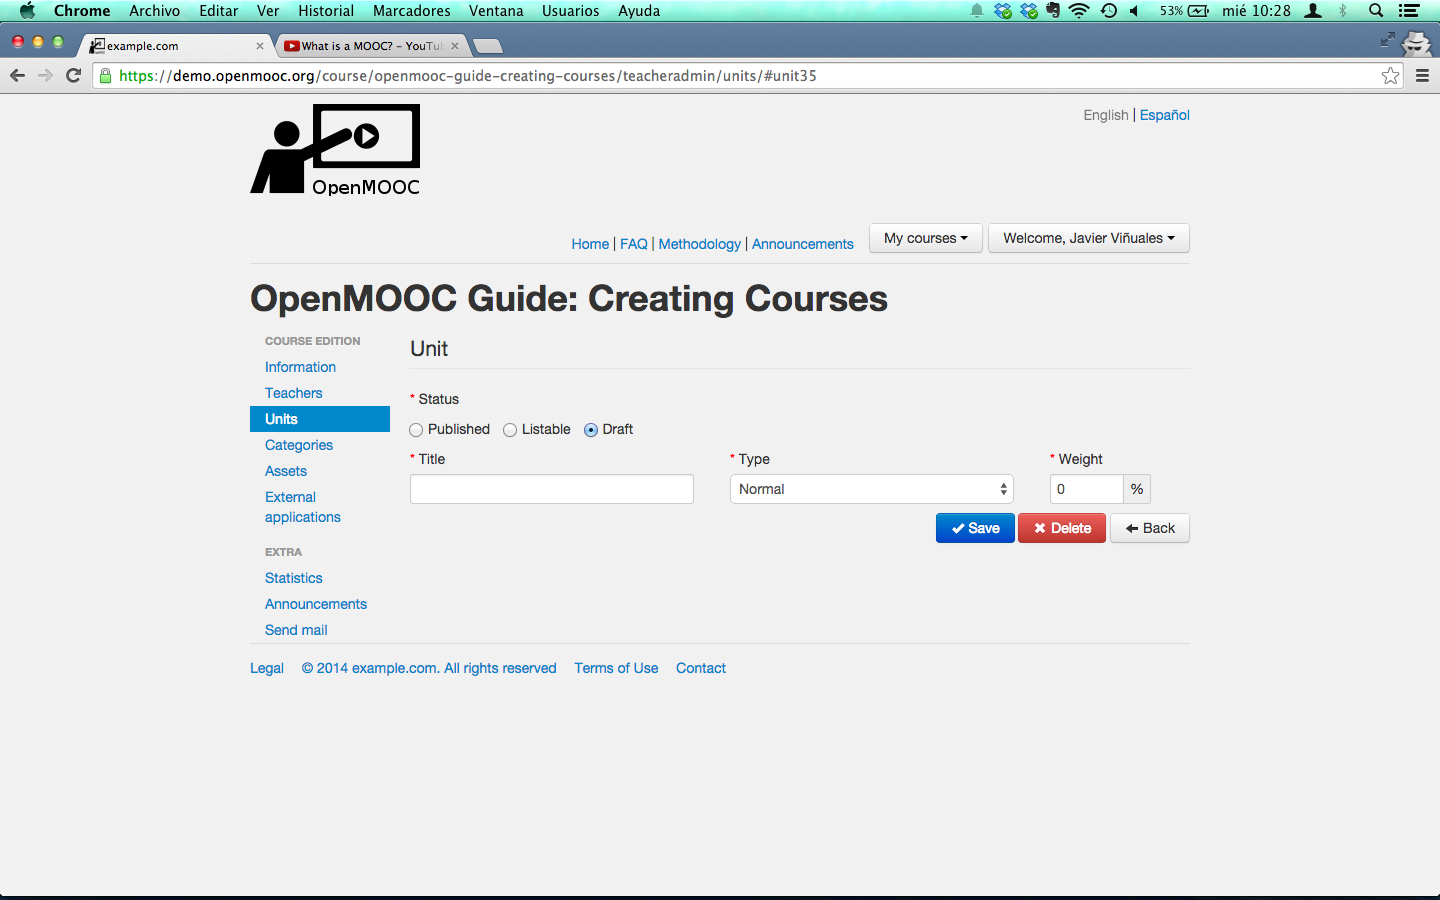
\includegraphics{4_course_units-2.png}

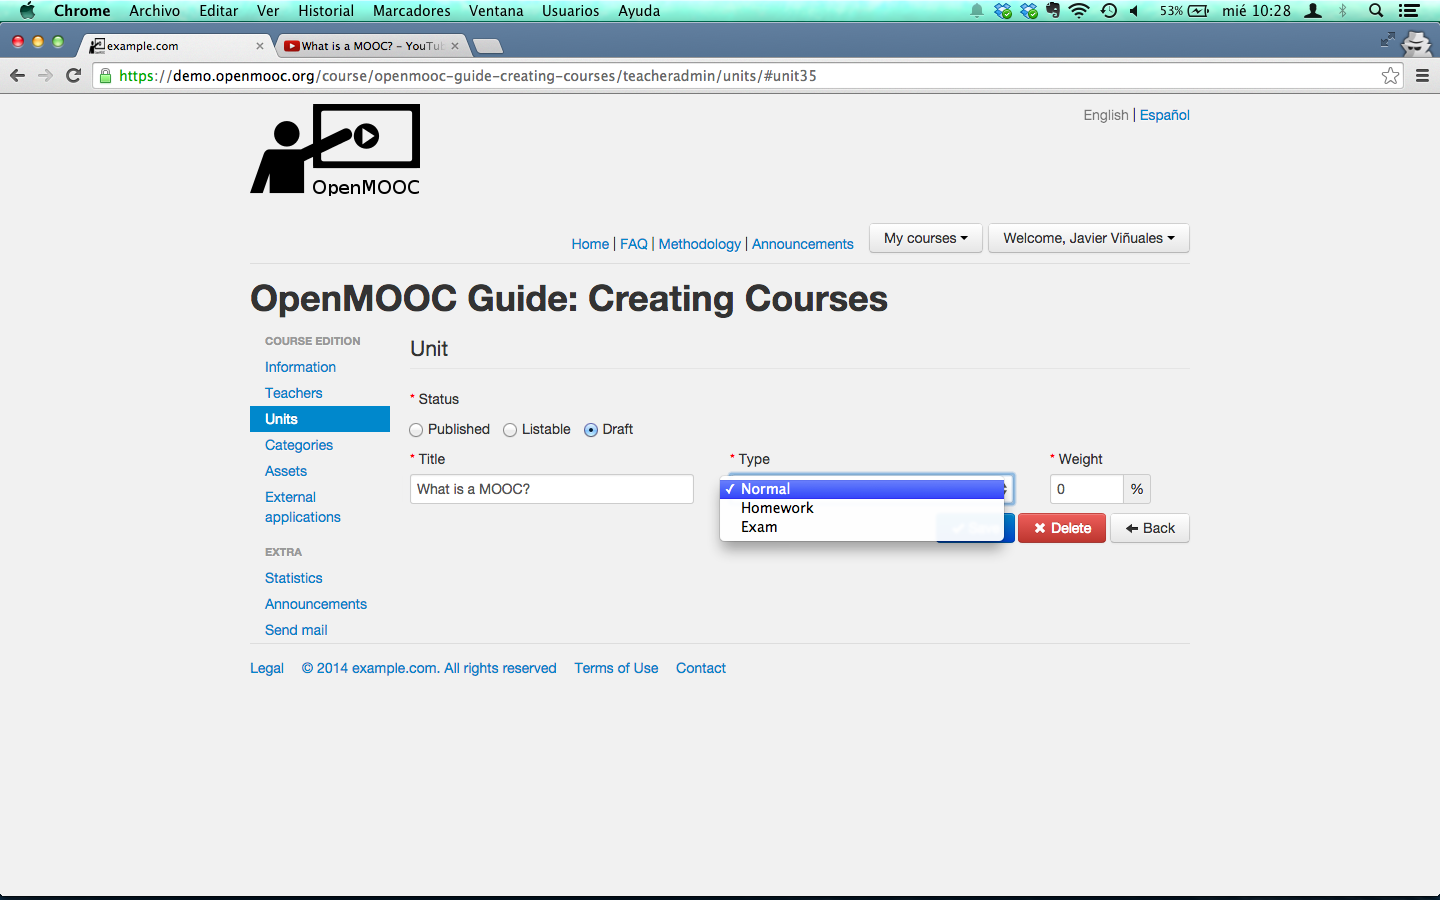
\includegraphics{4_course_units-3.png}

\item {} 
You will get a succes message from the platform and finally, you have to push the \textbf{save} button.

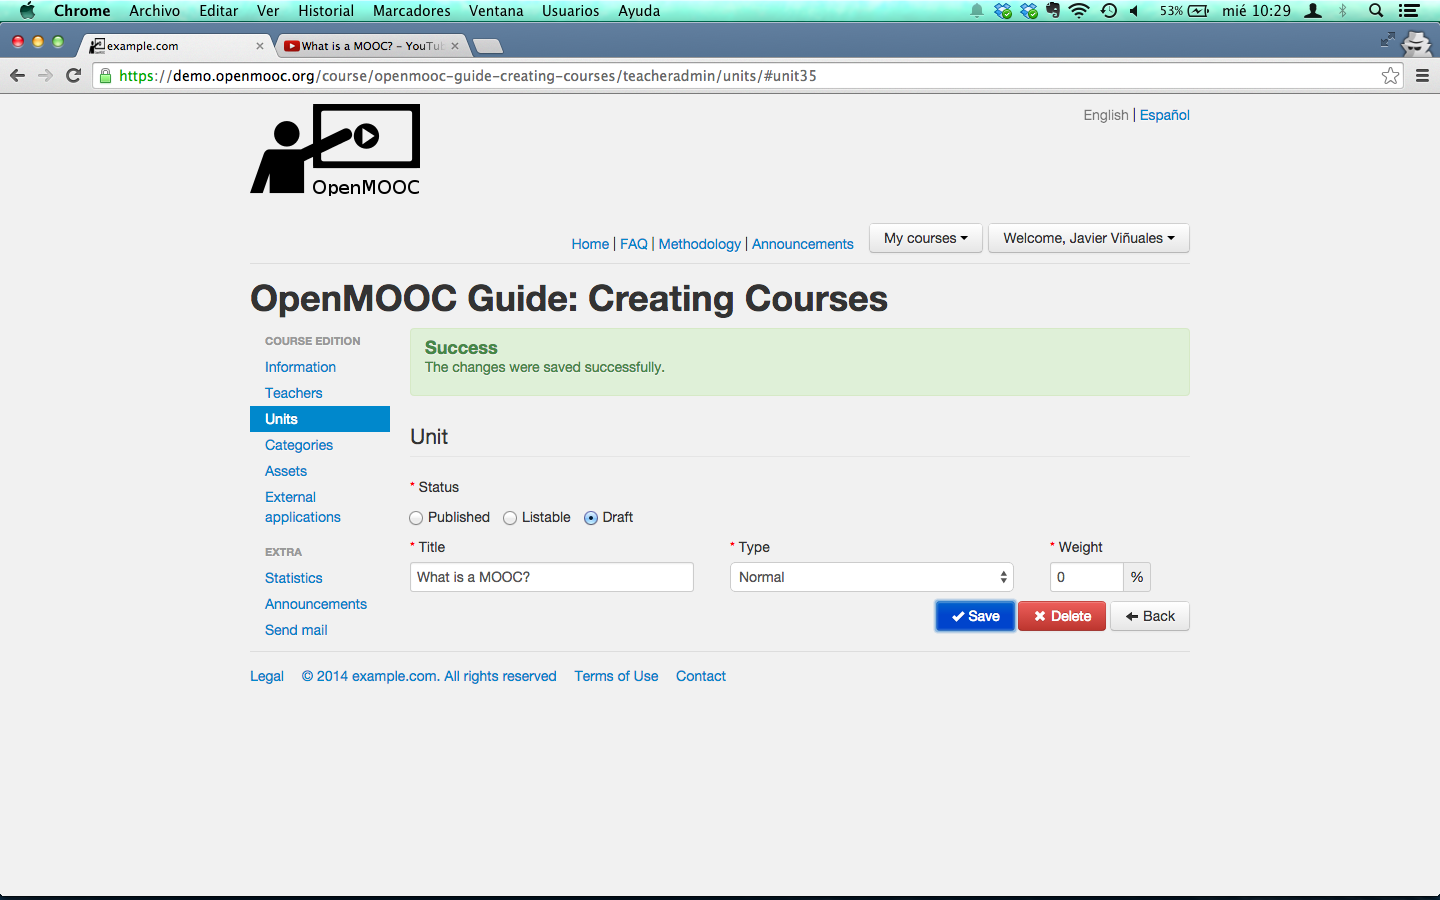
\includegraphics{4_course_units-4.png}

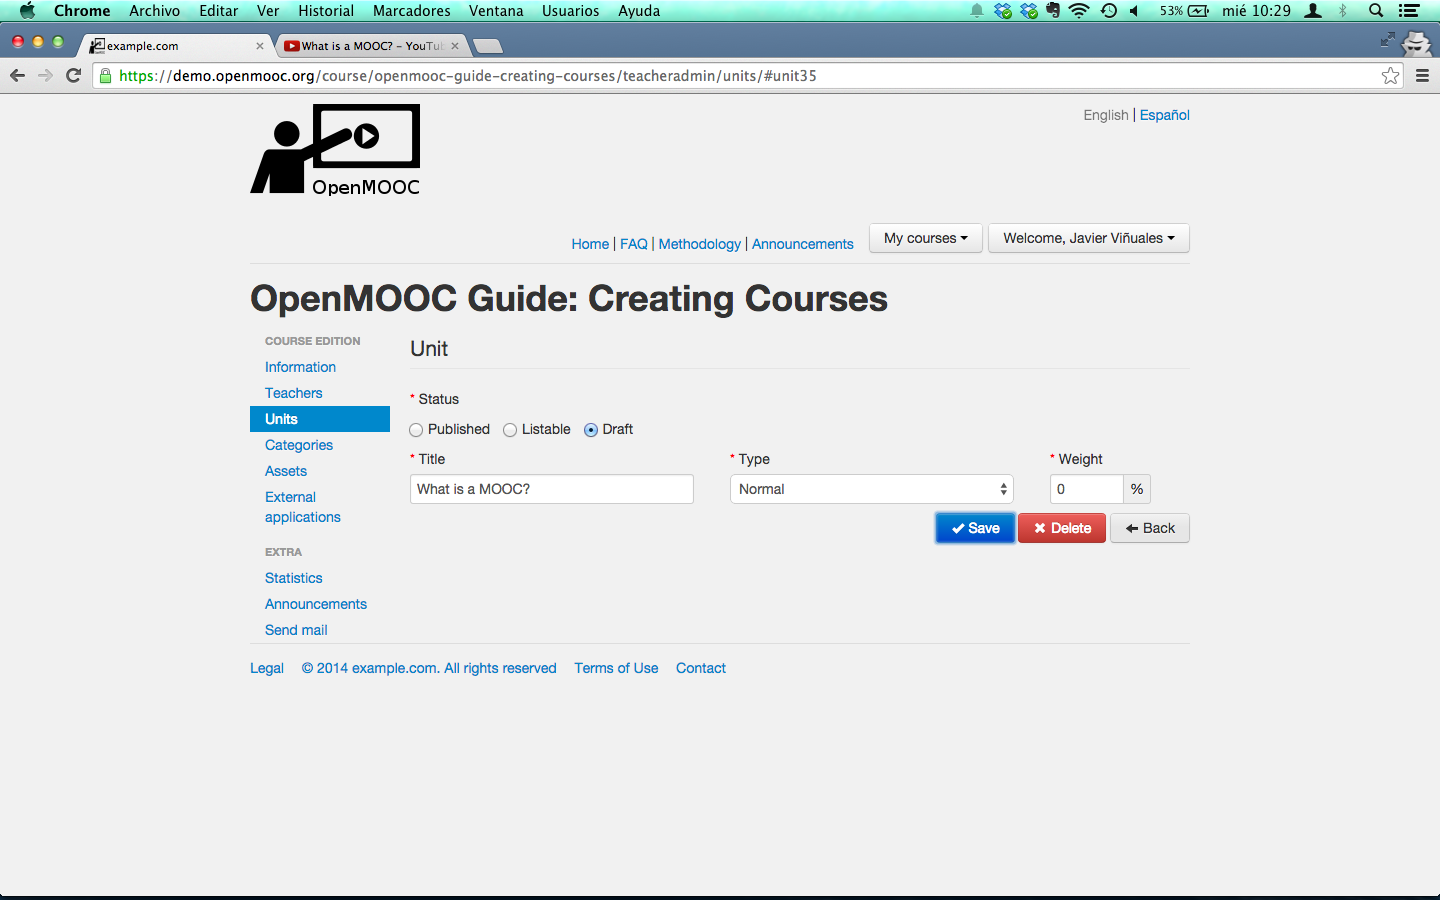
\includegraphics{4_course_units-5.png}

\item {} 
An empty box with the name of the unit you just created will be shown.

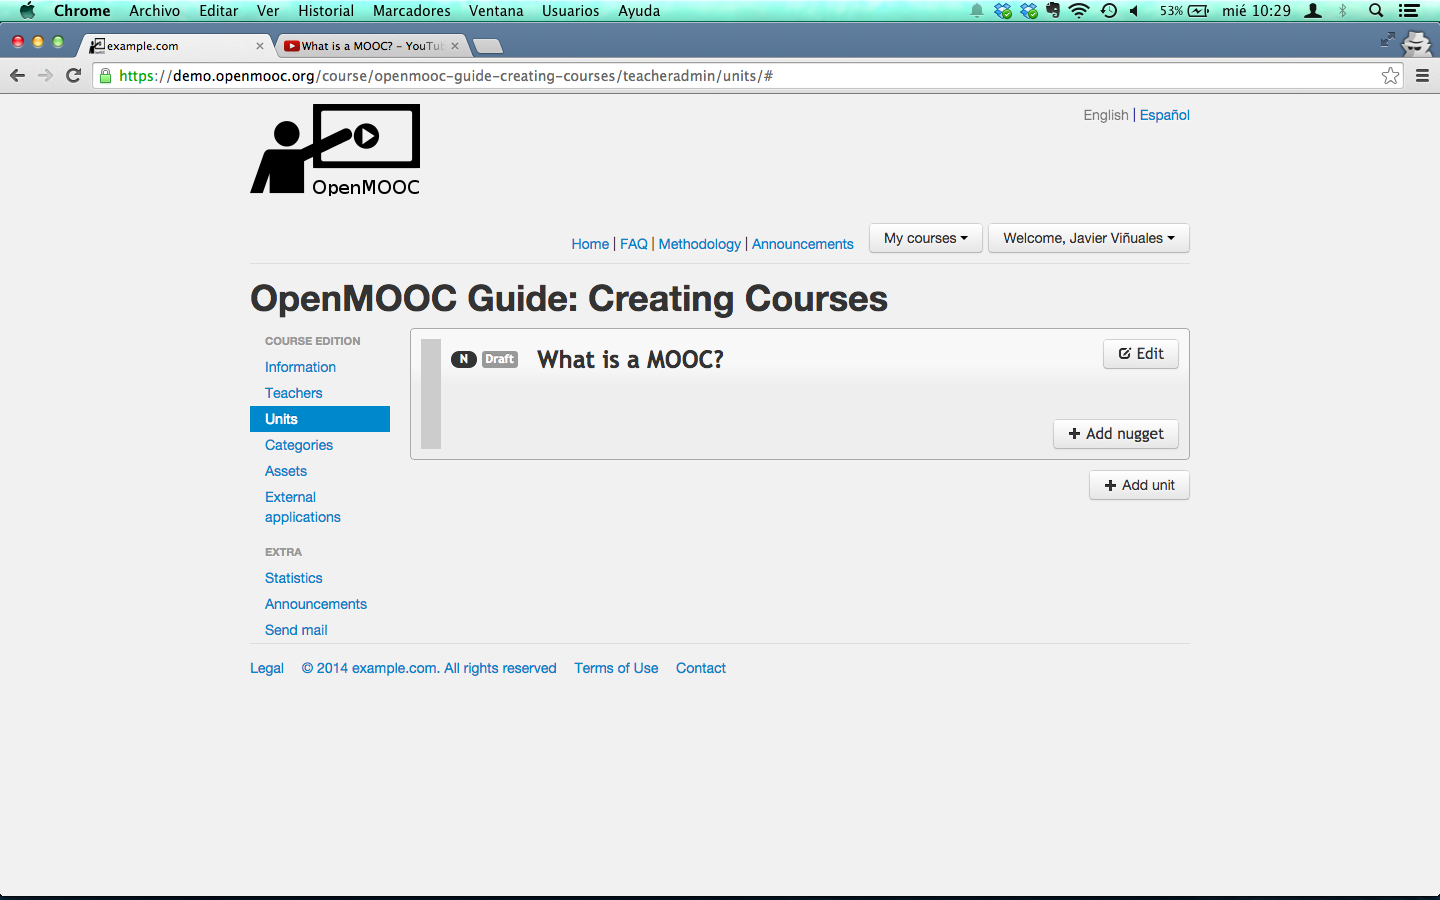
\includegraphics{4_course_units-6.png}

\item {} 
Now, you need to add a pill or nugget by clicking \textbf{Add nugget} button. Fill the title for the pill, select the online video server to use (p.e. Youtube), copy the URL for the video resource and paste it in the \textbf{Content id or url} text box. Finally, fill the text areas \textbf{Supplementary material} and \textbf{Instructor's comments}, and click \textbf{save} button.

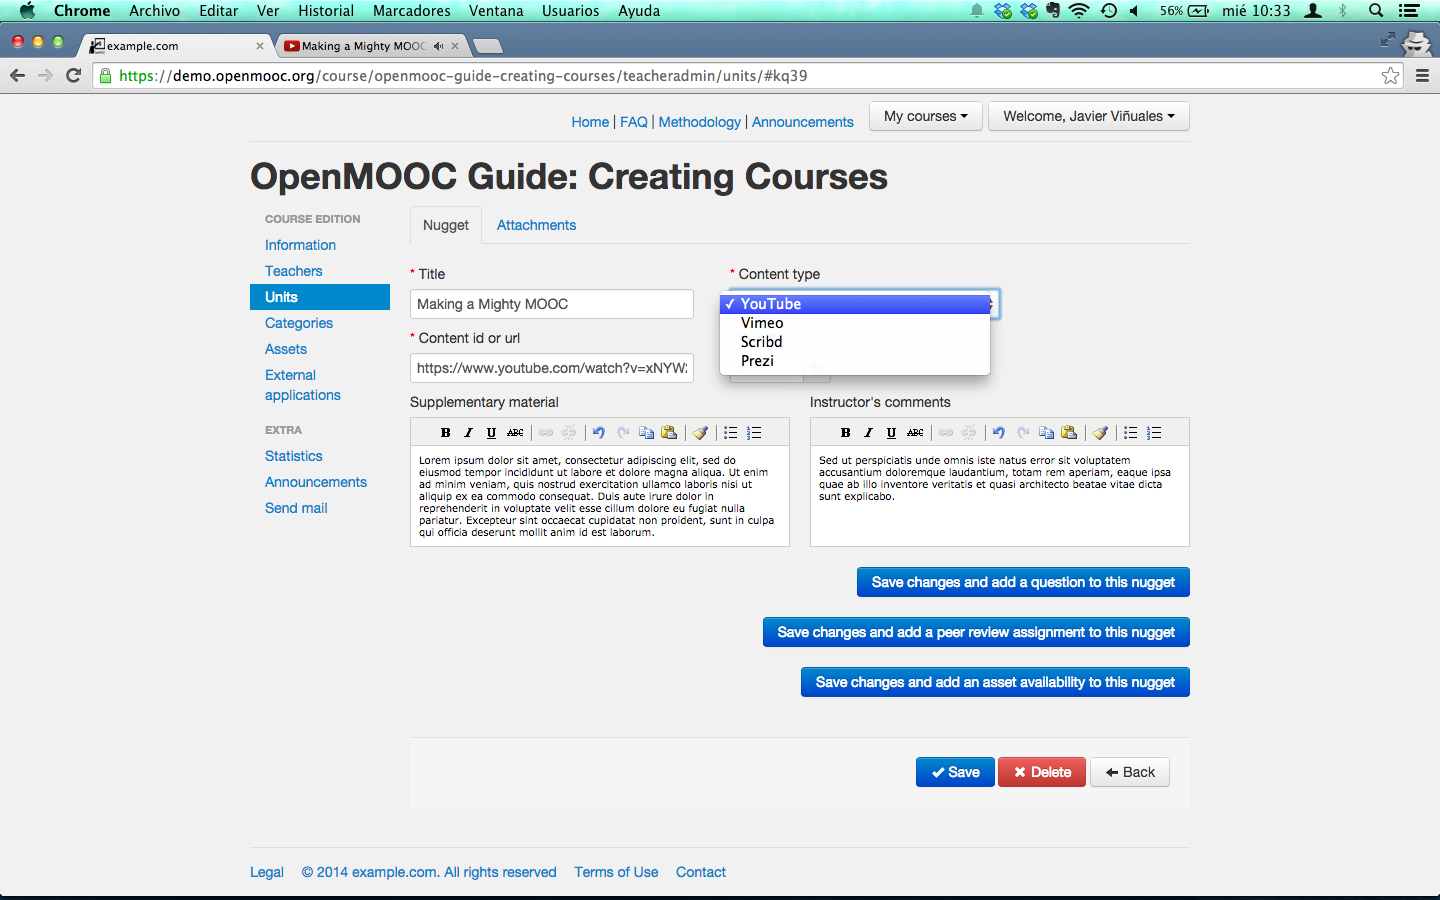
\includegraphics{4_course_units-7.png}

\item {} 
Do the same and you will see two pill into the Unit.

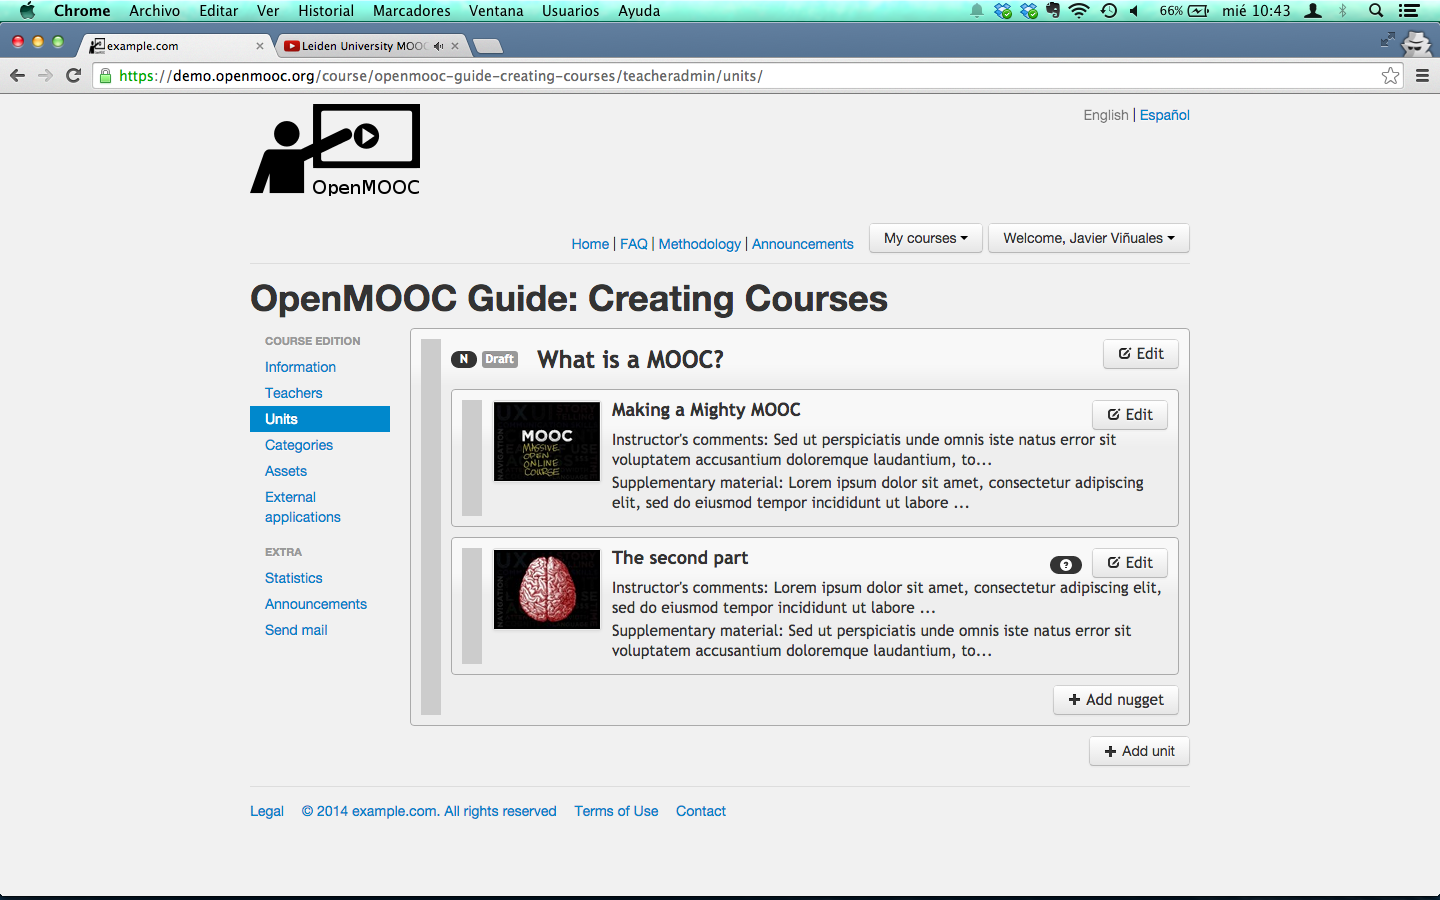
\includegraphics{4_course_units-8.png}

\item {} 
To add a question to an existing pill, you have to click on the \textbf{Edit} button. When you get the pill form, push the \textbf{Save changes and add a question to this nugget} button.

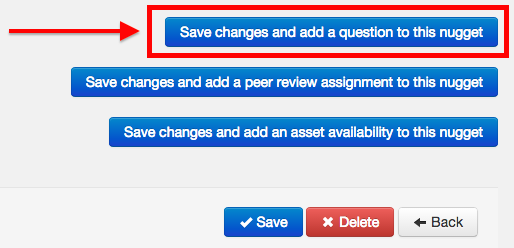
\includegraphics{4_course_units-9a.png}

\item {} 
The statement is always a video for a questionary, but not for peer review. You can use a blank canvas or the last frame if you're using for the stamment a Youtube video. You have to add question's solution like an online video (Youtube, Vimeo, Prezi or Scribd) or a text solution.

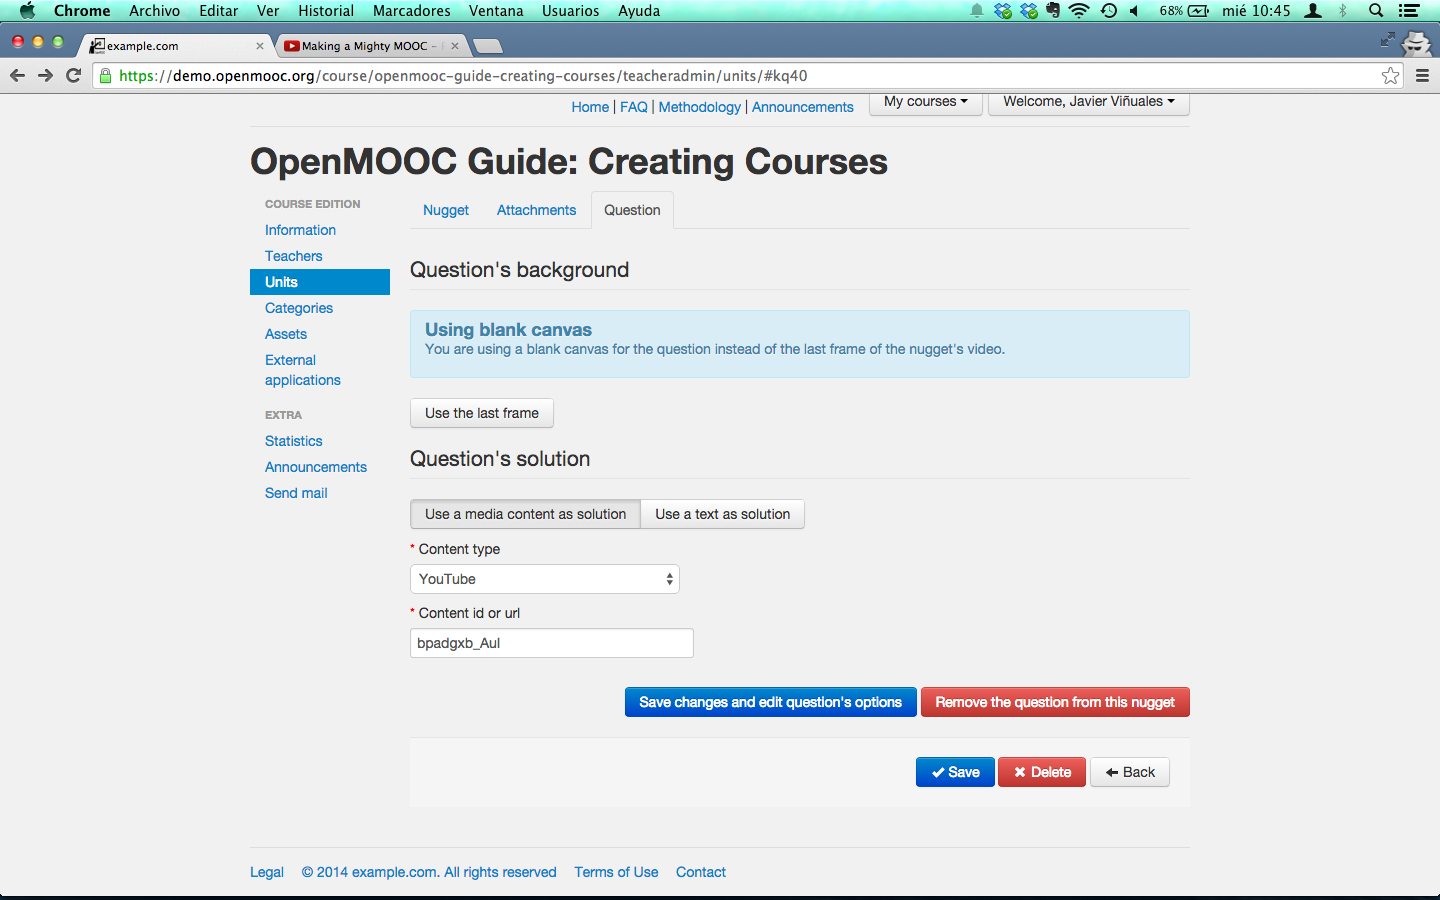
\includegraphics{4_course_units-9b.png}

\item {} 
OpenMOOC has a powerfull forms builder to open the possibilities of creating questions on a blank canvas or the last frame from a Youtube video. You can drag items out of the canvas form if you wish to remove. The form is automatically saved.

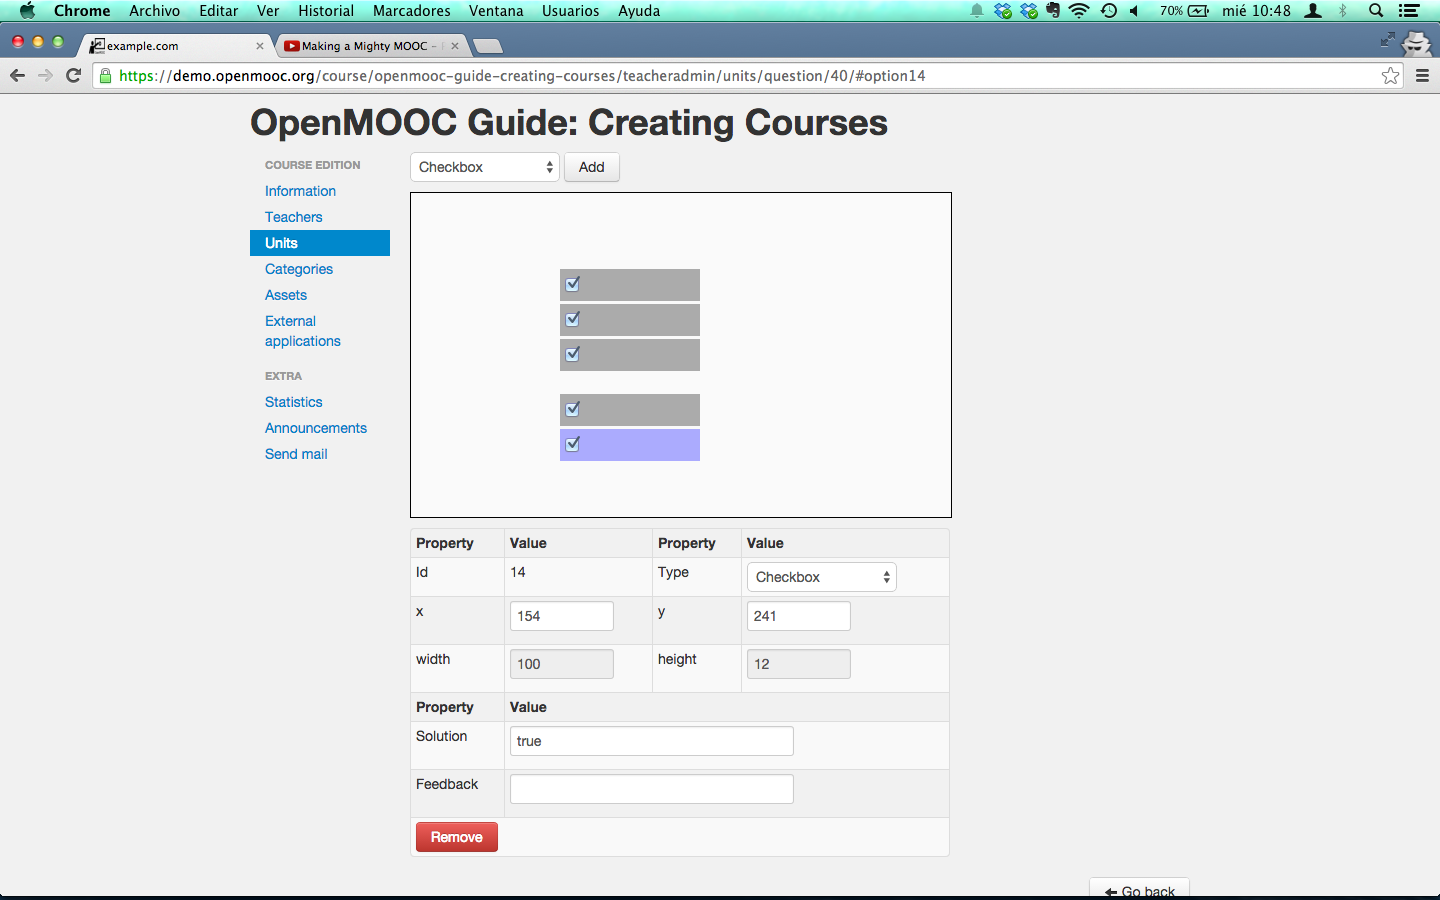
\includegraphics{4_course_units-10.png}

\item {} 
To create a peer review task you have to click on the \textbf{Edit} button of a pill and then, click on the \textbf{Save changes and add a peer review assingnment to this nugget}.

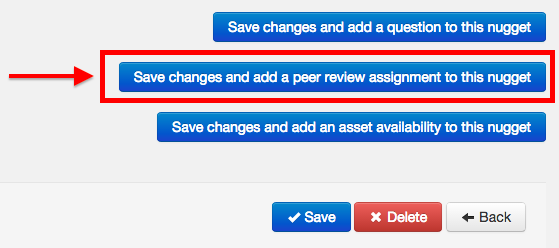
\includegraphics{4_course_units-11.png}

\item {} 
You have to add an assignment description and the minimum number of reviewers needed. Every student needs to send his peer assignment and review the minimun number of assignments from others students. It's an anonymous process.

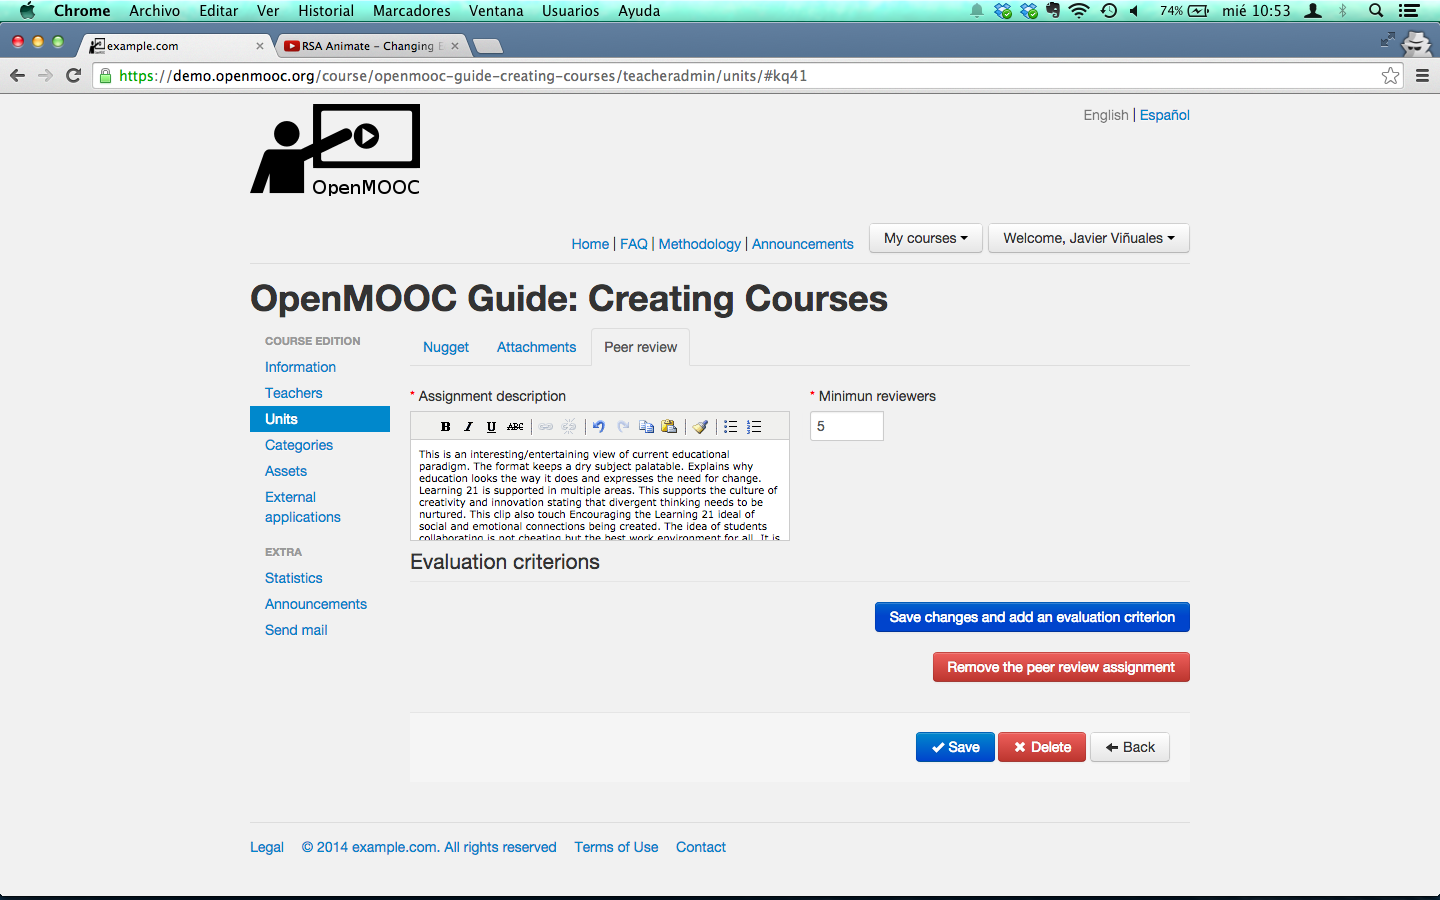
\includegraphics{4_course_units-12a.png}

\item {} 
Finally, you need to add some criteria to evaluate the work from other students. Every student will recieve the review tasks in a inbox into a panel named \textbf{Reviews}.

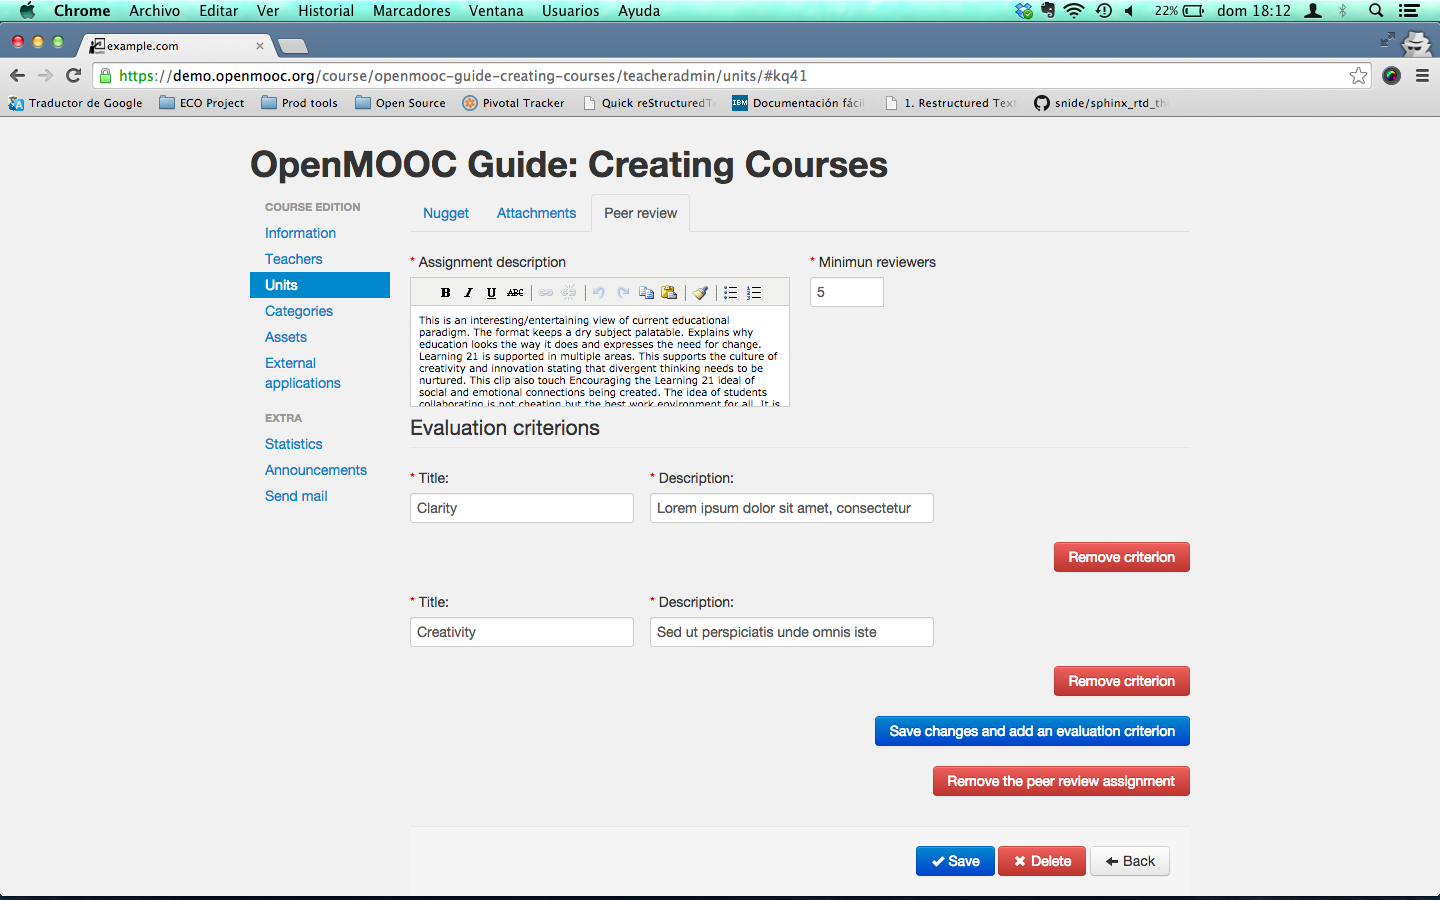
\includegraphics{4_course_units-12b.png}

\item {} 
This is the unit with pills you just created

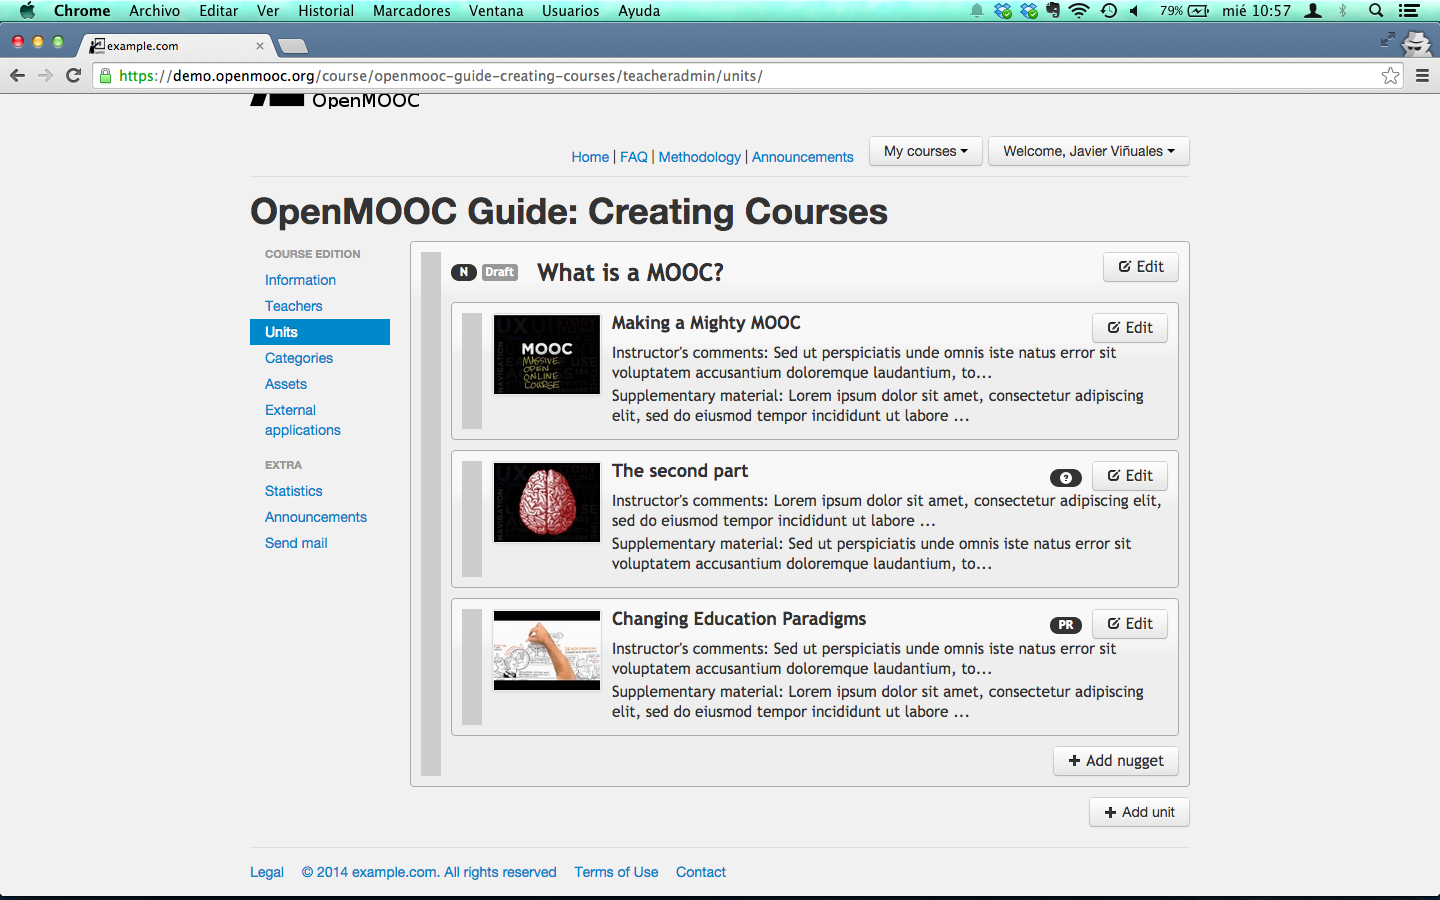
\includegraphics{4_course_units-13.png}

\end{enumerate}


\chapter{Categories}
\label{categories::doc}\label{categories:categories}\label{categories:id1}

\section{Overview}
\label{categories:overview}
The categories are like a tags and a course can be in multiple categories

\code{https://demo.openmooc.org/category/cat1/}

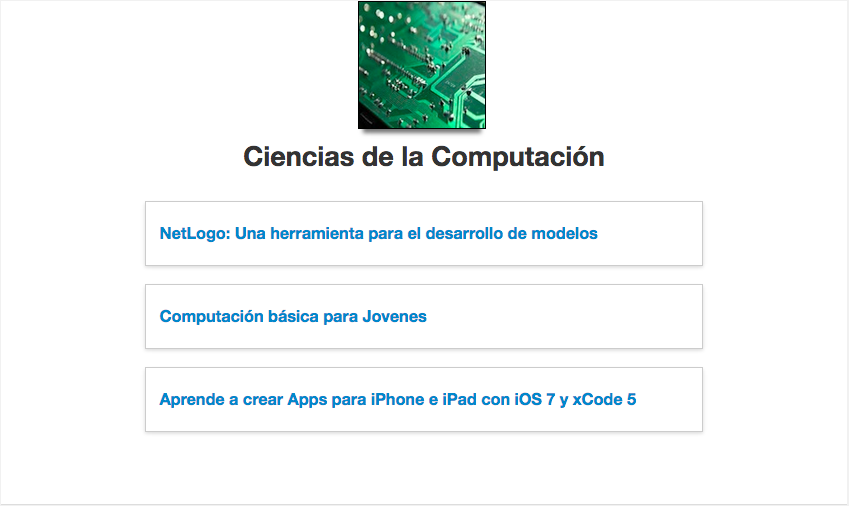
\includegraphics{5_categories-0a.png}

You can add more categories in the URL to filter a group of them like

\code{https://demo.openmooc.org/category/cat1/cat2/cat3}

Categories and the URL scheme used by OpenMOOC are very useful to be used to
promote the course and is optimal for search engine.

OpenMOOC not have categories by default, you must create them as an administrator to assign it to a course.


\section{Adding categories to a course}
\label{categories:adding-categories-to-a-course}\begin{enumerate}
\item {} 
You can add categories to the course. Some categories only can be added by the platform administrator.

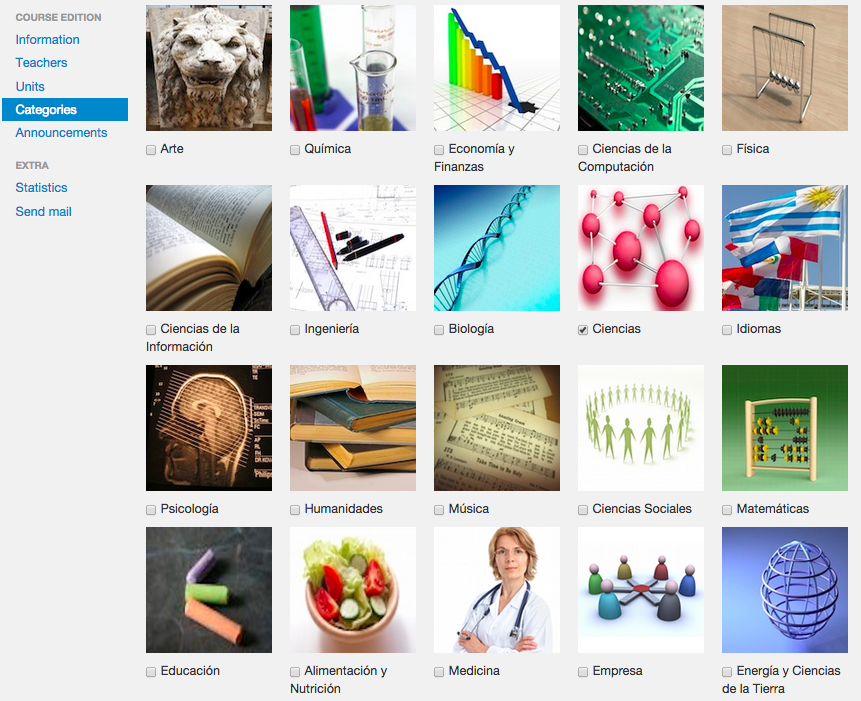
\includegraphics{5_categories-1.png}

\end{enumerate}


\section{Organization web page}
\label{categories:organization-web-page}
Some categories are used to group classes of an organization.
These categories can only be assigned to a course by the platform administrators.

\code{https://demo.openmooc.org/category/organization1/}

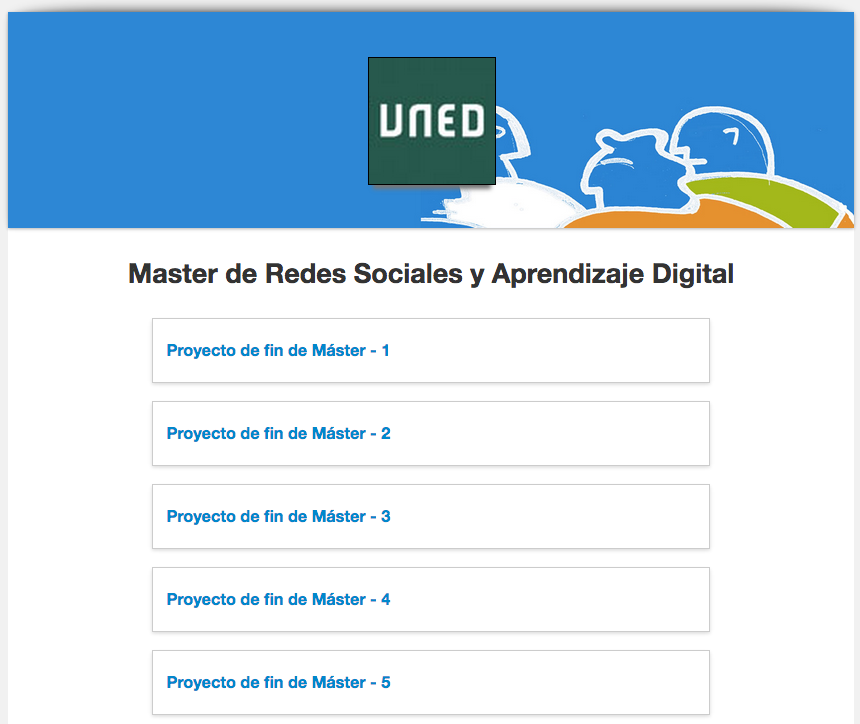
\includegraphics{5_categories-0b.png}

In this way, you get the organization page on the platform, with the list of courses.
The thumbnail image, the short description and start date will be shown for each course listed.



\renewcommand{\indexname}{Index}
\printindex
\end{document}
